\documentclass[energies,article,submit,moreauthors]{Definitions/mdpi}
\usepackage{tabularx}
\usepackage{array}
\firstpage{1}
\pubvolume{1}
\issuenum{1}
\articlenumber{0}
\pubyear{2026}
\copyrightyear{2026}
\datereceived{}
\daterevised{}
\dateaccepted{}
\datepublished{}
\Title{CARS-MODE: Constraint-Aware Repair and Strategy-Pool Multi-Objective Differential Evolution on a SimBench-Derived Mixed-Voltage Portfolio Proxy}
\Author{Linyao Zhang, Jieyun Zheng, Zhanghuang Zhang, Shiyuan Ni, Guilian Wu}
\AuthorNames{Linyao Zhang, Jieyun Zheng, Zhanghuang Zhang, Shiyuan Ni, Guilian Wu}
\address{Economic and Technological Research Institute of State Grid Fujian Electric Power Co., Ltd., Fuzhou 350000, Fujian, China}
\corres{Correspondence: zjy\_0701@163.com (J. Zheng)}
\abstract{Distribution utilities allocate limited budgets among reinforcement, distributed energy resources, storage, and automation. This optimizer study represents those choices with a SimBench-derived portfolio proxy, not action-aligned expansion decisions. CARS-MODE combines binary multi-objective differential evolution, adaptive parameters and mutation strategies, budget repair, and crowding. A 2940-run rerun covers six distinct configurations plus an independent base-configuration seed replication and exactly reproduces the archived hypervolumes. With equal configuration weight, CARS-MODE's sampled-bound/clipped hypervolume is 0.04240, 6.06\% above NSGA-II with returned-population repair. The audit nevertheless finds 2281 clipped coordinates among 68248 front points. Under unclipped analytic envelopes and reference 1.05, CARS-MODE scores 0.00043464 versus 0.00043530 for that baseline and ranks fourth; common-reference IGD+ ranks it fifth. FixedDE remains nominally ahead, so adaptation is unresolved. An archived composition-level AC check is illustrative: CARS-MODE changes 11 matched cases from infeasible to feasible and 3 in reverse, but these dependent fixed cases provide neither seed-level physical feasibility nor electrical superiority. The supported contribution is a reproducible configuration-sensitive screening and diagnostic workflow.}
\keyword{distribution-planning portfolio proxy; distributed energy resources; energy storage; multi-objective optimization; differential evolution; self-adaptive parameter control; constraint handling; SimBench}
\providecommand{\tightlist}{\setlength{\itemsep}{0pt}\setlength{\parskip}{0pt}}
\begin{document}
\section{Introduction}\label{introduction}

The distribution grid turns the energy transition into an investment problem. Photovoltaic connections, storage, and electrified loads are arriving faster than many medium- and low-voltage feeders were designed to accommodate. Distribution system operators must decide which feeders to reinforce, where to accept DER, where storage is justified, and which automation upgrades to fund under a limited budget. Each action changes cost, losses, voltage exposure, hosting capacity, and reliability. Because those quantities conflict, DER and storage planning is a recurring constrained multi-objective problem.

Evolutionary multi-objective algorithms are widely used in this literature, but two practical frictions persist. The first is algorithmic: differential evolution (DE) is sensitive to its control parameters and mutation strategy {[}1{]}, and the planning problem is binary, budget-constrained, and rugged. A single fixed DE configuration can therefore stall. Self-adaptive DE variants (jDE {[}2{]}, SaDE {[}3{]}) addressed this limitation on continuous benchmarks two decades ago, whereas many energy-planning studies still use either fixed-parameter DE or an off-the-shelf NSGA-II. The second friction is evidential: studies based on private networks or unchecked objective proxies are difficult to reproduce and easy to over-interpret. Comparative optimizer research emphasizes consistent evaluation protocols {[}4{]}. In this study, repeated-run statistical comparisons are therefore paired with an explicit power-flow check of the surrogate planning objectives.

CARS-MODE is a binary multi-objective DE with four implemented mechanisms grouped into three controls. It self-adapts each individual's scale factor \(F\) and crossover rate \(CR\) in the jDE manner. A success-driven pool selects between rand/1 and best/1 mutation, deterministic repair removes low-benefit actions until the budget is met, and crowding truncation preserves front diversity. The current FixedDE control disables the parameter controller and strategy pool jointly.

The evidence uses public data and reproducible implementations. SimBench deterministically supplies the benchmark {[}5{]}, while nine baselines and four ablations use real algorithm implementations, including pymoo references where available {[}6{]}. The archived standard hypervolume uses fixed method-independent sampled bounds; this revision also evaluates every preserved front with analytic feasible envelopes, a closer reference point, and common-reference IGD+. Every stochastic method uses 30 seeded runs and Holm-corrected Mann--Whitney tests; the deterministic Weighted Sum rule is compared descriptively.

The study uses a two-level evaluation. The planning objectives are engineering indices computed from SimBench subnet statistics---fast enough to support a rigorous statistical protocol, but proxies nonetheless. At the second level, one run-index-0 compromise-plan composition for each method present in the archived AC panel is mapped onto four real SimBench MV networks and checked with pandapower AC load flow {[}7{]} across six fixed operating cases (base, peak load, load growth, extreme growth, high DER infeed, and an \(N-1\) contingency). GDE3, NSDE, and NSGA-II+Repair were added after that panel and have no archived AC rows. The resulting disagreement between proxy ranking and electrical feasibility is an illustrative composition finding, not a seed-replicated method comparison.

Accordingly, this is an optimizer study on a SimBench-derived mixed-voltage portfolio proxy, not an action-aligned distribution expansion study. The candidate attributes are generated from subnet statistics, and the AC stage maps portfolio compositions onto separate networks rather than evaluating the optimizer's selected actions at their original nodes.

The contributions of this paper are:

\begin{enumerate}
\def\labelenumi{\arabic{enumi}.}
\tightlist
\item
  \textbf{A constraint-aware multi-objective DE framework with testable mechanism groups on a portfolio proxy.} CARS-MODE integrates jDE parameter control, a success-driven two-strategy pool, deterministic budget repair, and crowding diversity. Repair and diversity are removed individually; a combined control replaces adaptive parameters and the strategy pool with fixed \(F/CR\) and rand/1. The design therefore separates the framework-level proxy result from repair and diversity effects while testing parameter-and-strategy adaptation as a bundle (Section 4).
\item
  \textbf{A reproducible public mixed-voltage portfolio-proxy benchmark with an audited evaluation protocol.} Six deterministic planning configurations over at most 72 SimBench-derived candidate actions, with \texttt{pareto\_quality} retained as an independent seed replication of the base configuration rather than a seventh configuration; 30 seeds per stochastic method and seed block; all 2940 final fronts preserved; and an exact eight-decimal rerun of the archived hypervolume column (Sections 2 and 5). The benchmark does not provide nodal, monetarily calibrated expansion actions.
\item
  \textbf{Configuration-specific and reference-sensitive optimizer effects.} CARS-MODE's sampled-bound/clipped effect over NSGA-II+Repair is positive in all six configurations, but its analytic-HV effect is positive in three and its common-reference IGD+ effect in one. With equal configuration weight, NSGA-II+Repair is 0.15\% higher at analytic reference 1.05 and CARS-MODE ranks fourth; common-reference IGD+ ranks it fifth. The evidence therefore rejects a normalization-invariant superiority claim (Sections 6.1, 6.6, and 6.7).
\item
  \textbf{A bounded component and decision-screening analysis.} Removing repair or diversity retains large legacy-metric deficits, whereas FixedDE is nominally 0.60\% higher and leaves the combined adaptation bundle unresolved. The archived pandapower panel adds engineering screening value by exposing proxy--physics disagreement and matched changes relative to the same No-Plan cases, but it evaluates only three run-index-0 compositions per method and supplies neither optimizer-seed physical-feasibility uncertainty nor electrical results for the later direct controls (Sections 6.2--6.5).
\end{enumerate}

Section 2 reviews related work, and Sections 3--5 define the problem, method, and experimental protocol. Section 6 reports the optimization, ablation, AC-validation, and sensitivity results. Sections 7--9 discuss the findings, state the limitations, and conclude the paper.

\begin{center}\rule{0.5\linewidth}{0.5pt}\end{center}

\section{Related Work}\label{related-work}

Three threads frame this work: distribution network expansion planning with DER and storage, evolutionary and swarm metaheuristics in power system planning, and self-adaptive differential evolution with constraint handling.

\subsection{Distribution Network Expansion Planning with DER and Storage}\label{distribution-network-expansion-planning-with-der-and-storage}

Active distribution network planning has moved from single-objective conductor sizing to portfolio decisions that co-optimize reinforcement, DER siting, storage, and flexibility. Recent surveys map this shift: Prenc {[}8{]} catalogues the optimization principles applied in planning and operation of active distribution networks, and Salda\~{n}a-Gonz\'{a}lez et al.~{[}9{]} organize the elements of modern planning models, including the entry of generative-AI scenario tools. On the modeling side, robustness to uncertainty dominates: Liu et al.~{[}10{]} plan expansions under distributional uncertainty via Wasserstein-distance ambiguity sets and dual relaxation, and Wang et al.~{[}11{]} coordinate source--network--storage expansion against WGAN-GP-generated scenarios. Reliability-driven formulations add restoration and islanding to reinforcement choices {[}12{]}, while Ferreira et al.~{[}13{]} extend the planning boundary upward to the transmission--distribution interface, and Chen et al.~{[}14{]} specialize it to hybrid AC/DC campus networks for data centers. Closest to our task, He et al.~{[}15{]} co-optimize distribution networks with storage and electric vehicles using an improved NSGA-II, and Alrashidi et al.~{[}16{]} integrate DG, capacitor banks, and EV charging stations in radial feeders through a classification-based global optimization scheme.

Across this thread the algorithmic engine is almost always a Pareto-based genetic algorithm or a mathematical-programming reformulation; DE appears rarely, and when the engine is improved, the improvement is seldom isolated by ablation. Equally relevant to us is what these papers evaluate on: private or single test systems are the norm, and the mapping from optimization objective to AC feasibility is usually asserted rather than measured. Our study is designed to make this mapping explicit and measurable.

\subsection{Evolutionary and Swarm Metaheuristics in Power System Planning}\label{evolutionary-and-swarm-metaheuristics-in-power-system-planning}

The broader planning literature in energy venues provides many metaheuristic variants. Qi et al.~{[}17{]} apply enhanced beluga whale optimization to vulnerability-driven storage planning; Demirbas et al.~{[}18{]} develop an enhanced coati algorithm for static and dynamic transmission expansion; and Cadena-Albuja et al.~{[}19{]} compare DE with other optimizers for energy-limited economic dispatch. Two recurring limitations motivate our protocol. First, hybrid or ``improved'' algorithms are not always accompanied by mechanism controls, making the source of added value difficult to identify. We therefore isolate repair and diversity and test the parameter-and-strategy controller against a combined fixed control. Second, independent runs, rank-based tests, and standard indicators such as hypervolume {[}20{]} are applied unevenly in some application studies, and benchmarking audits document the associated reproducibility risks {[}4,21,22{]}. We use a standard indicator, 30 seeded runs, and Holm-corrected non-parametric tests so that single-digit percentage differences can be distinguished from seed variation.

\subsection{Self-Adaptive Differential Evolution and Constraint Handling}\label{self-adaptive-differential-evolution-and-constraint-handling}

DE {[}1{]} owes much of its practical success to parameter adaptation and constraint handling. jDE {[}2{]} encodes \(F\) and \(CR\) in each individual and resamples them with a small probability per generation. SaDE {[}3{]} additionally learns mutation-strategy probabilities from recent successes; Das and Suganthan {[}23{]} review this lineage. Success-history adaptation (SHADE) {[}24{]} and composite strategy--parameter schemes {[}25{]} extend the same principle, while Ahmad et al.~{[}26{]} survey recent developments. Multi-objective DE variants place these mechanisms under Pareto selection, commonly using non-dominated sorting and crowding {[}27{]} or decomposition {[}28{]}. Constraint-handling alternatives include penalties, feasibility-first domination, and repair {[}29,30{]}. Repair is especially attractive for knapsack-like budgets because it returns evaluations to the fundable region.

The reviewed studies provide limited evidence on combining jDE/SaDE-style adaptation and greedy budget repair inside a binary multi-objective DE for distribution-planning portfolios and then inspecting the resulting plans with AC power flow. Our controls isolate repair and diversity and compare the full controller with a fixed-parameter, single-strategy alternative. Because the latter changes two adaptive subcomponents together, it tests their joint contribution rather than identifying either one separately. The AC check is important because adaptation is commonly justified by indicator gains alone; here the joint proxy-level contrast is unresolved, while the selected compromise plans show a favorable but exploratory electrical pattern (Section 6.3).

\subsection{Gap Statement}\label{gap-statement}

In summary, distribution-planning studies supply the task context but do not consistently isolate algorithmic components or validate proxy objectives electrically. Metaheuristic studies supply algorithmic variants, while the DE literature supplies adaptation mechanisms, but their combination in budget-constrained binary planning with power-flow validation remains limited. Table 1 compares these features in representative recent works. This paper studies that intersection through a reproducible self-adaptive multi-objective DE, component-level ablations, repeated statistical tests, and a separate AC inspection that explicitly reports disagreement with the proxy ranking.

\begin{table*}[t]
\centering
\scriptsize
\setlength{\tabcolsep}{3pt}
\caption{Feature comparison with representative related work. "yes" = present; -- = absent by design; n.r. = not reported in the cited work; n/a = not applicable to the study's scope.}\label{tab:1}
\begin{tabularx}{\textwidth}{@{}>{\raggedright\arraybackslash}X >{\raggedright\arraybackslash}X >{\raggedright\arraybackslash}X >{\raggedright\arraybackslash}X >{\raggedright\arraybackslash}X >{\raggedright\arraybackslash}X >{\raggedright\arraybackslash}X >{\raggedright\arraybackslash}X@{}}
\toprule
Work & Task & Engine & Pareto front returned & Self-adaptive $F$/$CR$ / strategy & Constraint repair & Per-component ablation & Objective proxy checked by AC power flow \\
\midrule
jDE [2] & continuous benchmarks & DE & -- & yes / -- & -- & -- & n/a \\
SaDE [3] & continuous benchmarks & DE & -- & yes / yes & -- & -- & n/a \\
SHADE [24] & continuous benchmarks & DE & -- & yes / -- & -- & -- & n/a \\
He et al. [15] & distribution planning (storage, EV) & improved NSGA-II & yes & n.r. & feasibility constraints & n.r. & n.r. \\
Alrashidi et al. [16] & DG/CB/EVCS planning & classification-based global optimization & -- (aggregated objective) & n.r. & n.r. & n.r. & n.r. \\
Qi et al. [17] & resilience-driven storage planning & enhanced beluga whale optimization & yes & n.r. & n.r. & n.r. & n.r. \\
Demirbas et al. [18] & transmission expansion & enhanced coati optimization & n.r. & n.r. & n.r. & n.r. & n.r. \\
Cadena-Albuja et al. [19] & economic dispatch & DE (comparative study) & -- & n.r. & n.r. & n.r. & n/a \\
CARS-MODE (this work) & distribution planning portfolios & binary multi-objective DE & yes & yes / yes & yes (greedy budget repair) & repair/diversity separate; adaptive bundle joint & yes (pandapower, four MV networks) \\
\bottomrule
\end{tabularx}
\end{table*}

\subsection{Companion Project, Shared Generators, and Independent Question}\label{companion-project-shared-generators-and-independent-question}

The companion project \texttt{mintou\_p4\_shield\_resilience\_planning} belongs to the same research program. It and this study share the generators used to derive SimBench-based benchmark inputs. That generator layer is common infrastructure, not an independent dataset or a replication of either paper's results. The CARS-MODE question is independent: under a fixed proxy benchmark, comparison budget, and evaluation protocol, does the complete constrained-search framework improve proxy-front quality relative to the implemented controls, and which mechanism groups survive ablation? The companion project instead concerns resilience-oriented stress-scenario screening in the evaluation layer. Results and conclusions in this paper are restricted to the CARS-MODE optimizer question.

\begin{center}\rule{0.5\linewidth}{0.5pt}\end{center}

\section{Problem Formulation and Public Benchmark}\label{problem-formulation-and-public-benchmark}

\subsection{Planning Portfolios as Multi-Objective Binary Selection}\label{planning-portfolios-as-multi-objective-binary-selection}

Let \(\mathcal{A} = \{a_1, \dots, a_n\}\) be a pool of candidate planning actions. Each action belongs to one of four kinds---feeder \textbf{reinforcement}, \textbf{storage} installation, \textbf{DER} installation, and \textbf{automation}---and carries synthetic cost \(c_i\), four P3 objective-benefit attributes, and two inherited fields (resilience gain and DER-support score). A plan is a binary vector \(x \in \{0,1\}^n\). The planner minimizes five objectives simultaneously:

\[
\min_{x \in \{0,1\}^n} F(x) = \big( C(x),\; L(x),\; U(x),\; -H(x),\; -R(x) \big),
\]

where \(C\) is total synthetic cost, \(L\) a network loss index, \(U\) a voltage-risk index, \(H\) the DER hosting-capacity index, and \(R\) a reliability index; all five are analytic functions of selected-action attributes and the planning configuration's fixed load factor (Section 3.2 gives their provenance). The single hard constraint is the budget:

\[
\textstyle\sum_i c_i x_i \le B, \qquad v(x) = \max\big(0, (\textstyle\sum_i c_i x_i - B)/B\big),
\]

with \(B = 980\) synthetic cost units at the nominal level and experiment-specific factors 0.82, 1.00, or 1.20. The budget is the only hard constraint. Voltage risk and hosting capacity remain objectives because their target levels are not jointly satisfiable within this proxy budget; treating them as constraints would incorrectly label every method infeasible. Any residual target shortfall is therefore reported as a property of the compromise portfolio rather than hidden inside the feasibility definition.

A plan \(x\) dominates \(x'\) when it is no worse in all five objectives and better in at least one. The feasible non-dominated front contains mutually non-dominating plans that respect the budget. Hypervolume measures the normalized objective-space volume dominated by that front relative to a fixed reference point, rewarding both convergence and spread {[}20{]}.

\subsection{Benchmark Construction from SimBench}\label{benchmark-construction-from-simbench}

All problem data derive from the public SimBench complete mixed dataset (\texttt{1-complete\_data-mixed-all-0-sw}) {[}5{]}. Active and reactive load, renewable capacity, line length, line count, and average maximum loading are aggregated from \texttt{Load.csv}, \texttt{Line.csv}, and \texttt{RES.csv}. The 18 subnetworks with the highest combined load and line-length stress are retained (Table 2).

Each subnet contributes one action of each kind, yielding \(n=72\) candidates. Reinforcement cost scales with line length and load. Storage and DER gains scale with the shortfall from a renewable target of 55\% of load, while automation reliability gain scales with line count. All rules are implemented in code; no attribute is assigned manually per candidate.

The candidate pool spans EHV to LV subnets, whereas Section 5.4 validates compositions on four separate MV networks. Thus the proxy provides portfolio statistics and the AC stage evaluates action mixes on concrete lower-voltage grids. The mapping is compositional rather than nodal, and both tiers belong to the same SimBench family.

\begin{table*}[t]
\centering
\footnotesize
\setlength{\tabcolsep}{3pt}
\caption{Benchmark source profile.}\label{tab:2}
\begin{tabularx}{\textwidth}{@{}>{\raggedright\arraybackslash}X >{\raggedright\arraybackslash}X@{}}
\toprule
Property & Value \\
\midrule
SimBench network & \texttt{1-complete\_data-mixed-all-0-sw} (EHV--LV complete mixed) \\
Subnetworks used & 18 (EHV1, HV1, HV2, LV3.101--LV3.107, LV3.201--LV3.208) \\
Candidate actions & 72 (18 subnets x 4 kinds) \\
Total load & 71,348.9 MW \\
Total installed RES & 12,234.9 MW \\
Total line length & 34,296.2 km \\
Nominal budget $B$ & 980 cost units (synthetic, not monetarily calibrated) \\
\bottomrule
\end{tabularx}
\end{table*}

\textbf{Complete candidate contract.} For subnet \(s\), the source aggregates are active load \(P_s\) {[}MW{]}, reactive load \(Q_s\) {[}MVAr{]}, load count \(N_s^{L}\) {[}count{]}, installed renewable capacity \(G_s\) {[}MW{]}, line length \(D_s\) {[}km{]}, line count \(N_s^{\ell}\) {[}count{]}, and mean recorded maximum loading \(\bar\rho_s\) {[}percent{]}. Only subnets with \(P_s>0\) and \(N_s^{\ell}>0\) are eligible. The implementation ranks them by the mixed-unit proxy \(P_s+0.2D_s\) and retains the first 18. This ranking is a deterministic data-reduction heuristic, not a physical stress index. Define

\[
\sigma_s=\frac{P_s}{\max(0.2,D_s)},\qquad
d_s=\max(0,0.55P_s-G_s).
\]

The constant 0.55 defines a synthetic renewable-gap target used only to generate attributes; it is not presented as a grid-code, utility, or policy threshold. For every retained subnet, the deterministic generator creates four attribute tuples in the order \((c,a^L,a^U,a^H,a^R,a^S,a^{\mathrm{DER}})\):

\begin{itemize}
\tightlist
\item
  reinforcement: \[
  (60+4.5D_s+7P_s,\ 0.012D_s+0.020\sigma_s,\ 0.020+0.006\sigma_s,\ 0.06d_s,\ 0.018N_s^{\ell},\ 0.016N_s^{\ell},\ 0.20);
  \]
\item
  storage: \[
  (50+16\sqrt{P_s+1},\ 0.025\sqrt{P_s+1},\ 0.018\sqrt{\sigma_s+1},\ 0.12d_s+0.08P_s,\ 0.055\sqrt{N_s^L+1},\ 0.070\sqrt{N_s^L+1},\ 0.80);
  \]
\item
  DER: \[
  (45+10\sqrt{P_s+1},\ 0.018\sqrt{P_s+1},\ 0.012,\ 0.18d_s+0.10P_s,\ 0.020\sqrt{N_s^L+1},\ 0.028\sqrt{N_s^L+1},\ 1.00);
  \]
\item
  automation: \[
  (38+1.8N_s^{\ell},\ 0.006N_s^{\ell},\ 0.010\sqrt{\sigma_s+1},\ 0.025d_s,\ 0.085\sqrt{N_s^{\ell}+1},\ 0.115\sqrt{N_s^{\ell}+1},\ 0.35).
  \]
\end{itemize}

The coefficients convert the physical source columns into \textbf{synthetic proxy points}: only \(c\) has synthetic cost units, \(a^{\mathrm{DER}}\) is a dimensionless support score, and the five planning benefits plus the inherited resilience benefit are dimensionless index contributions. Consequently, the expressions must not be read as MW, MWh, reliability hours, or monetary estimates. \(Q_s\) and \(\bar\rho_s\) are retained in the source profile but do not enter the P3 candidate or objective equations.

The P3 objective mapping is also deterministic. Let \(P_\Sigma=\sum_sP_s\), \(D_\Sigma=\sum_sD_s\), and let \(\lambda_e\) be the load factor of planning configuration \(e\). The baseline indices and hosting denominator are

\[
L_0=0.12+0.015\frac{D_\Sigma}{\max(1,P_\Sigma)},\qquad
U_0=0.18+0.010\frac{P_\Sigma}{\max(1,D_\Sigma)},\qquad
D_H=0.08P_\Sigma.
\]

For a decoded plan \(x\), the five minimized proxy objectives are

\[
\begin{aligned}
C(x)&=\sum_j c_jx_j,\\
L_e(x)&=\max\!\left(0.015,L_0\lambda_e-\frac{\sum_j a_j^Lx_j}{120}\right),\\
U_e(x)&=\max\!\left(0.005,U_0\lambda_e-\frac{\sum_j a_j^Ux_j}{10}\right),\\
H_e(x)&=\min\!\left(1,\frac{\sum_j a_j^Hx_j}{\max(1,D_H)}\right),\\
R_e(x)&=\min\!\left(1,0.35+\frac{\sum_j a_j^Rx_j}{28}\right),\\
F_e(x)&=(C(x),L_e(x),U_e(x),-H_e(x),-R_e(x)).
\end{aligned}
\]

The floors 0.015 and 0.005 and the caps at 1 are part of the proxy definition, not observed engineering limits. The generated resilience gain \(a^S\) is not a P3 objective, but the shared implementation does use it in the repair and deterministic Weighted Sum scores (Sections 4.3 and 5.1); omitting that fact would make those procedures irreproducible. A separate descriptive DER-readiness index is

\[
D^{\mathrm{DER}}(x)=\min\!\left(1,
\frac{\sum_j a_j^{\mathrm{DER}}x_j}{0.62\max(1,\sum_jx_j)}\right).
\]

Neither \(D^{\mathrm{DER}}\) nor the generated resilience attribute enters hypervolume. Hosting and DER-readiness shortfalls are exported only for the selected compromise as \([t_H-H_e(x)]_+\) and \([t_D-D^{\mathrm{DER}}(x)]_+\); the targets are descriptive and never become feasibility gates or method-specific scores.

We state plainly what this construction is: a \emph{reproducible public proxy} for portfolio-level distribution planning. The objective indices are engineering-plausible functions of real network statistics, not AC power-flow results --- which is exactly why Section 6.3 validates the outcome plans with pandapower load flow, and why Section 8 lists the remaining distance to an engineering-grade planning claim.

\subsection{Deterministic Planning Configurations and Base Replication}\label{deterministic-planning-configurations-and-base-replication}

Six distinct configurations exercise the pool along three axes---candidate-pool composition, load factor, and budget tightness---with an identical reporting protocol (Table 3). The archive contains seven experiment-labelled seed blocks because \texttt{pareto\_quality} is a second optimizer-seed block for the base configuration. It is replication within the same deterministic problem, not an additional configuration. Both the proxy operating point and the later AC stress cases are deterministic; stochasticity comes only from the optimizer seed for methods that use random variation.

\begin{table*}[t]
\centering
\scriptsize
\setlength{\tabcolsep}{3pt}
\caption{Six deterministic planning configurations. The base row contains two independently seeded optimizer blocks; every other row contains one.}\label{tab:3}
\begin{tabularx}{\textwidth}{@{}>{\raggedright\arraybackslash}X >{\raggedright\arraybackslash}X >{\raggedright\arraybackslash}X >{\raggedright\arraybackslash}X >{\raggedright\arraybackslash}X >{\raggedright\arraybackslash}X >{\raggedright\arraybackslash}X >{\raggedright\arraybackslash}X@{}}
\toprule
Configuration & Archived seed block(s) & Budget factor & Load factor $\lambda_e$ & Search dimension $n$ & Pool restriction & $t_H$ & $t_D$ \\
\midrule
Base & base\_distribution\_planning; pareto\_quality (internal replicate) & 1.00 & 1.0 & 72 & none & 0.018 & 0.48 \\
DER-only pool & der\_siting\_sizing & 1.00 & 1.0 & 54 & storage candidates excluded before all methods run & 0.025 & 0.56 \\
Storage-only pool & storage\_allocation & 1.00 & 1.0 & 54 & DER candidates excluded before all methods run & 0.025 & 0.56 \\
Load growth & load\_growth\_expansion & 1.00 & 1.3 & 72 & none & 0.025 & 0.48 \\
Tight budget & constraint\_repair & 0.82 & 1.0 & 72 & none & 0.018 & 0.48 \\
Loose budget & runtime\_scalability & 1.20 & 1.0 & 72 & none & 0.018 & 0.48 \\
\bottomrule
\end{tabularx}
\end{table*}

The two base seed blocks use method-specific seed streams derived by hashing their archived experiment and method identifiers. They are pooled only for the base row's descriptive configuration mean; the two blocks remain separate in the upstream inferential tables. The two budget variants (0.82x, 1.20x) probe the tight- and loose-budget regimes. The ``runtime scalability'' identifier is retained from an earlier benchmark version but used only for its budget role, and no runtime-scaling claim is made.

Terminology is fixed as follows. A \textbf{planning configuration} is one of the six deterministic proxy problems in Table 3 and contains exactly one objective-evaluation operating point \((\lambda_e,1,0)\) for load, DER, and outage multipliers. A \textbf{seed block} is an archived experiment label that supplies 30 method-specific optimizer seeds; the base configuration has two. A \textbf{seeded run} is one stochastic optimizer repetition within a seed block, and its seed does not create a load or outage scenario. An \textbf{AC operating case} in Section 5.4 is one fixed combination of validation network and load/DER/\(N-1\) setting. Those AC cases are deterministic stress tests, not random scenarios or independent optimizer replications. The shared configuration class serializes inherited ranges for load \((0.95,1.25)\), DER \((0.7,1.3)\), and outage \((0,0.25)\), and the shared module defines a 16-scenario constant, but the P3 branch bypasses all four settings and returns the single point above; they generate no P3 scenario samples. \texttt{use\_expected\_loss} is false in every P3 configuration, so the loss objective is \(L_e\), not an outage-weighted expected-loss variant. The values \(t_H\) and \(t_D\) are implementation-recorded descriptive targets used only to export shortfalls. The available evidence does not supply a utility-calibration rationale for 0.018/0.025, 0.48/0.56, or the 55\% renewable-gap constant; they are disclosed benchmark design choices and do not affect feasibility, hypervolume, or compromise selection.

\begin{center}\rule{0.5\linewidth}{0.5pt}\end{center}

\section{CARS-MODE}\label{cars-mode}

Figure 1 summarizes one generation and separates adaptive search from feasibility and evaluation. Parameter and strategy updates act on the continuous population; decoding and deterministic budget repair produce binary plans; constraint-dominated environmental selection updates the population and archive; and AC validation is applied only to archived compromise plans after optimization.

\begin{figure*}[t]
\centering

\includegraphics[width=0.94\textwidth]{figures/fig_architecture.png}
\caption{CARS-MODE architecture. The feedback arrow denotes the next generation. Standard hypervolume and AC power-flow validation are readouts of the archived solutions and do not affect strategy-success updates.}\label{fig:1}
\end{figure*}

CARS-MODE is a binary multi-objective DE with explicit switches for repair and crowding diversity and one \textbf{joint} switch for parameter-and-strategy adaptation. Accordingly, NoRepair and NoDiversity are operator controls, FixedDE is a combined controller control, and NoDER is a search-space variant; the latter two cannot identify individual adaptive effects. The continuous genome has dimension \(n=72\) except in the two 54-candidate planning configurations. Initially \(g_{ij}\sim U(0,0.45)\), after which each coordinate is independently overwritten with \(0.75\) with probability 0.08. Thus approximately 8\% of initial coordinates decode as selected.

\textbf{Formal definitions.} A real genome \(g_i\in[0,1]^n\) is decoded into a binary phenotype and assigned normalized budget violation

\[
x_{ij}=\mathbb I[g_{ij}>0.5],\qquad
v(x_i)=\max\!\left(0,\frac{\sum_{j=1}^{n}c_jx_{ij}-B}{B}\right).
\]

The strict \(>0.5\) decoder is the CARS-MODE and Standard-DE rule. GDE3 and NSDE use the implementation's \(\geq0.5\) decoder, and the Boolean algorithms do not require a threshold. If repair changes \(x_i\), it does \textbf{not} write the removed bits back to \(g_i\); environmental selection stores the selected continuous genome together with its repaired phenotype, and the genome is decoded and repaired again after later variation.

The implementation uses one joint resampling gate \(Z_i\sim\operatorname{Bernoulli}(\tau)\) per individual and generation:

\[
F_i'=\begin{cases}0.1+0.8U_1,&Z_i=1,\\F_i,&Z_i=0,\end{cases}
\qquad
CR_i'=\begin{cases}U_2,&Z_i=1,\\CR_i,&Z_i=0,\end{cases}
\]

with independent \(U_1,U_2\sim U(0,1)\). Thus \(F_i\) and \(CR_i\) are either both redrawn or both retained. For each target, \(r_1,r_2,r_3\) are sampled without replacement from the population; the implementation does not separately exclude the target index \(i\). The two mutation candidates are

\[
m_i^{\mathrm{rand}}=g_{r_1}+F_i'(g_{r_2}-g_{r_3}),
\]

\[
m_i^{\mathrm{best}}=g_b+F_i'(g_{r_2}-g_{r_3}),\qquad g_b\in\mathcal F_1,
\]

where \(g_b\) is sampled uniformly from the first constraint-dominated front (feasible members precede infeasible ones). Binomial crossover forces one randomly selected coordinate to come from the mutant, and the resulting trial is clipped coordinate-wise:

\[
u_{ij}=\begin{cases}\operatorname{clip}(m_{ij},0,1),&
U_{ij}<CR_i'\ \text{or}\ j=j_{\mathrm{rand}},\\
g_{ij},&\text{otherwise}.
\end{cases}
\]

The strategy masses start at \((s_{\mathrm{rand}}^{(0)},s_{\mathrm{best}}^{(0)})=(1,1)\). If \(n_k^{(t)}\) trials generated by strategy \(k\) strictly improve their paired parents in generation \(t\), the exact update and next-generation probability are

\[
s_k^{(t+1)}=\max\!\left(0.2,0.95\,[s_k^{(t)}+n_k^{(t)}]\right),
\qquad
p_k^{(t+1)}=\frac{s_k^{(t+1)}}{s_{\mathrm{rand}}^{(t+1)}+s_{\mathrm{best}}^{(t+1)}}.
\]

A paired trial is credited when its violation is lower by more than \(10^{-12}\), or when violations agree within \(10^{-12}\) and it is no worse in every proxy objective and strictly better in at least one. Because the success counter is updated before multiplication by 0.95, the decay applies to both the previous mass and the current successes.

For an over-budget decoded plan, repair repeatedly removes

\[
b_j=\frac{a_j^L}{0.12}+\frac{a_j^U}{0.02}+\frac{a_j^H}{5}
+\frac{a_j^R}{2}+\frac{a_j^S}{2},\qquad
q_j=\frac{b_j}{\max(c_j,1)},\qquad
j^-=\operatorname*{arg\,min}_{j:x_j=1}q_j
\]

until the raw cost is no greater than \(B\). The denominators \((0.12,0.02,5,2,2)\) are the exact fixed repair weights. They were not learned, tuned by method, or justified by a monetary calibration; they scale heterogeneous proxy gains for this benchmark. DER-support is absent from repair, while the inherited resilience attribute is included. If several selected actions have the same minimum score, NumPy's first minimum is removed: the lowest candidate index, where candidates follow retained-subnet rank and the within-subnet order reinforcement, storage, DER, automation. Constraint dominance is defined by

\[
x\prec_c y\iff
[v(x)=0<v(y)]\ \lor\
[v(x)=v(y)=0\land x\prec_P y]\ \lor\
[v(x),v(y)>0\land v(x)<v(y)].
\]

Environmental sorting treats \(v\leq10^{-12}\) as feasible. Final reporting uses the slightly looser numerical filter \(v\leq10^{-9}\), removes duplicate binary plans, and retains the non-dominated objective rows. In the last partially admitted front, standard crowding distance is sorted in descending order; equal distances have no additional scientific tie criterion and follow the array order returned by NumPy. The NoDiversity control instead uses a seeded random permutation for this truncation.

Finally, with clipped normalized objective vector \(z(x)\) and fixed reference point \(r\), reported hypervolume is

\[
HV(\mathcal P;r)=\lambda_Q\!\left(\bigcup_{x\in\mathcal P}
[z_1(x),r_1]\times\cdots\times[z_Q(x),r_Q]\right).
\]

\subsection{jDE Self-Adaptive Control Parameters}\label{jde-self-adaptive-control-parameters}

The two control arrays \((F_i,CR_i)\) are initialized at \((0.5,0.9)\) and updated together: in every generation, the joint gate redraws \(F_i\sim U(0.1,0.9)\) and \(CR_i\sim U(0,1)\) with probability \(\tau=0.1\) {[}2{]}. A source-level detail limits the usual ``per-individual'' interpretation: environmental selection reorders the genomes and phenotypes, but the implementation does not apply the survivor indices to the \(F/CR\) arrays. The controls therefore persist by population slot, not as heritable fields attached to the selected genome. The sensitivity study in Section 6.4 sweeps \(\tau\) and finds a flat response. This controller and the strategy pool share the FixedDE switch, so that control estimates neither feature separately.

\subsection{Success-Driven Two-Strategy Pool}\label{success-driven-two-strategy-pool}

Mutation chooses between DE/rand/1 (a uniformly drawn base vector) and DE/best/1 (a base vector drawn from the current feasible-first non-dominated front), with probabilities proportional to recent success masses {[}3{]}. A trial is successful if it constraint-dominates its parent through lower violation or, at equal violation, Pareto improvement. Success masses decay by 0.95 per generation and have a floor of 0.2, preventing either strategy from being excluded. The pool combines exploratory rand/1 with the more intensive best/1 and lets observed successes determine their sampling probabilities.

\subsection{Constraint-Aware Budget Repair}\label{constraint-aware-budget-repair}

Every decoded plan that exceeds the budget is repaired deterministically using the fixed \(q_j\) score and candidate-index tie rule above. The selected action with the lowest score is removed repeatedly until the plan is affordable. This avoids spending selection slots on penalty-carrying phenotypes and concentrates search near the budget boundary. The 0.82x planning configuration directly stresses this mechanism.

\subsection{Crowding-Based Diversity Preservation}\label{crowding-based-diversity-preservation}

Environmental selection is elitist (\(\mu + \lambda\)): parents and trials are pooled, sorted by constraint-domination fronts, and truncated to the population size with crowding distance {[}27{]} breaking ties in the last admitted front. The corresponding ablation replaces crowding with a random tie-break. \emph{Motivation:} with only 40 individuals covering a five-objective front, losing spread control collapses the front to a few clusters---the ablation quantifies the equal-configuration legacy-HV loss as 33.32\% (Section 6.2).

\subsection{Algorithm Summary}\label{algorithm-summary}

\begin{verbatim}
CARS-MODE(pool, budget, seed):
  n <- 72, or 54 after an experiment-level kind exclusion
  initialize 40 genomes U(0,0.45); overwrite each gene by 0.75 with prob 0.08
  initialize F_i=0.5, CR_i=0.9 and strategy masses (1,1)
  decode with x_j = I[g_j > 0.5]; repair phenotype only            # 4.3
  for gen = 1 .. 40:
    evaluate current repaired phenotypes and form constraint fronts
    for each individual i:
      with one prob-0.1 gate, resample both slot controls F_i, CR_i # 4.1
      pick strategy rand/1 or best/1 by success mass               # 4.2
      mutate + forced-binomial crossover; clip genome to [0,1]
      decode trial with strict >0.5; repair phenotype only          # 4.3
    credit paired constraint improvements; decay/floor masses       # 4.2
    (mu+lambda) selection: constraint-domination NDS + crowding    # 4.4
    carry each selected genome together with its repaired phenotype
    retain F/CR by array slot (the source does not reorder them by survivor)
  deduplicate final feasible phenotypes and return their ND front
\end{verbatim}

\begin{center}\rule{0.5\linewidth}{0.5pt}\end{center}

\section{Experimental Setup}\label{experimental-setup}

\subsection{Methods Compared}\label{methods-compared}

Table 4 lists the fourteen methods: CARS-MODE, nine baselines, and four ablations. NSGA-II, NSGA-II with returned-population repair, MOEA/D, GDE3, and NSDE are pymoo implementations {[}6{]}. GDE3 and NSDE operate in \([0,1]^n\) and decode with \(g_j\geq0.5\); Standard DE and CARS-MODE use the strict \(g_j>0.5\) rule. GA, binary PSO {[}31{]}, and Standard DE optimize the same equally weighted normalized scalarization with a violation penalty. Weighted Sum is a deterministic greedy point rule. All final plans are evaluated by the method-independent proxy objectives, but their search-time constraint handling differs as disclosed below.

\begin{table*}[t]
\centering
\scriptsize
\setlength{\tabcolsep}{3pt}
\caption{Methods.}\label{tab:4}
\begin{tabularx}{\textwidth}{@{}>{\raggedright\arraybackslash}X >{\raggedright\arraybackslash}X >{\raggedright\arraybackslash}X@{}}
\toprule
Method & Role & Description \\
\midrule
CARS-MODE & proposed & binary MODE: jDE self-adaptive F/CR + two-strategy pool + budget repair + crowding \\
NSGA-II & baseline & pymoo NSGA-II, binary encoding, constrained \\
NSGA-II+Repair & baseline & constrained NSGA-II; the same deterministic budget repair is applied only to its returned population \\
MOEA/D & baseline & pymoo MOEA/D, budget as penalty \\
GDE3 & baseline & generalized differential evolution with constraint domination and fixed binary decoding \\
NSDE & baseline & nondominated-sorting differential evolution with fixed binary decoding and sampled $F$ \\
Standard DE & baseline & binary DE/rand/1/bin, fixed F = 0.5, CR = 0.9, scalarized \\
PSO & baseline & binary PSO (sigmoid velocity), scalarized \\
GA & baseline & single-objective GA, tournament + uniform crossover, scalarized \\
Weighted Sum & baseline & weighted-benefit greedy fill under budget \\
Ablation-FixedDE & ablation & joint control: $F = 0.5$, $CR = 0.9$, and only rand/1; parameter and strategy adaptation are both off \\
Ablation-NoRepair & ablation & budget repair disabled; feasibility-first constraint domination remains active \\
Ablation-NoDiversity & ablation & crowding replaced by random tie-break \\
Ablation-NoDER & ablation & DER and storage candidates removed from the search pool \\
\bottomrule
\end{tabularx}
\end{table*}

Ablation-NoDER is a \emph{problem-variant} probe rather than an operator switch. DER and storage columns receive search-only cost \(10^9\) and are zeroed by a Boolean mask after search; final objective evaluation and normalization use the original full experiment pool. By contrast, the \texttt{der\_siting\_sizing} and \texttt{storage\_allocation} exclusions in Table 3 remove one action kind from the problem for \textbf{every} method before search, leaving 54 variables. NoDER leaves only reinforcement and automation selectable (36 variables in either full or restricted experiment) and cannot support component attribution.

\textbf{Baseline encoding, constraint, and constant contract.} The shared scalar score used by GA, PSO, and Standard DE is

\[
S(x)=\sum_{q=1}^{5}\frac{f_q(x)-\ell_q}{\max(u_q-\ell_q,10^{-9})}+10v(x),
\]

with the fixed bounds from Section 5.3 and no clipping of these search scores. Their single returned best plan is repaired once after search before the feasible-front calculation. GA uses row-wise initial density \(U(0.03,0.18)\), binary tournaments of size 2, coordinate-wise uniform crossover probability 0.5, bit-flip probability \(1.5/n\), and elitist best-40 replacement. PSO uses the same initial-density range, initial velocity \(N(0,0.1)\), inertia 0.72, cognitive and social coefficients 1.49, velocity clipping to \([-6,6]\) before the logistic transform, and personal/global-best replacement under \(S\). Standard DE uses the CARS-MODE sparse initialization, DE/rand/1/bin with \(F=0.5\), \(CR=0.9\), one forced mutant coordinate, genome clipping to \([0,1]\), and the strict decoder.

NSGA-II uses one explicit inequality \(G=v(x)\) with Boolean two-point crossover and bit-flip mutation. Their probabilities were not overridden, and the available run configuration does not pin a pymoo version; exact library-default probabilities therefore cannot be certified as archival constants. NSGA-II+Repair runs that same constrained search and repairs only the returned population. GDE3 uses DE/rand/1/bin with \(F=0.5\), \(CR=0.9\) and \(G=v(x)\); NSDE uses the same variant and \(CR=0.9\) with pymoo's sampled \(F\in[0.3,0.9]\), also with \(G=v(x)\). MOEA/D uses 35 Das--Dennis reference directions (five objectives, three partitions), 10 neighbors, neighbor-mating probability 0.7, and the Boolean operators; because this pymoo configuration does not expose an inequality constraint, it minimizes \(F(x)+10^4v(x)\mathbf 1\) instead. These are configuration-specific controls, not claims about the algorithm families in general.

The deterministic Weighted Sum rule sorts by the \textbf{un-divided} benefit \(b_j\) defined in Section 4 (not \(q_j\)), then scans that order and adds an action only if its cost fits the remaining budget. Its five fixed benefit scales are therefore \((0.12,0.02,5,2,2)\), including resilience and excluding DER support. Equal benefits have no authored secondary criterion; the implementation uses the order returned by NumPy's descending \texttt{argsort}. This point rule is feasible by construction and has one effective output per seed block.

\subsection{Protocol}\label{protocol}

Each stochastic method runs \textbf{30 independently derived seeds} per archived seed block. For zero-based run index \(h\), the implementation computes the SHA-1 digest of \texttt{p3\textbar{}experiment\textbar{}method} and sets

\[
\operatorname{seed}(h)=200000+7919h+\big(\operatorname{int}(\text{first six hex digits},16)\bmod4096\big).
\]

Thus method cells do not share a random stream. The archive has \(14\times(6\text{ configurations}+1\text{ base replicate})\times30=2940\) rows: 2730 seeded stochastic runs and 210 repeated invocations of Weighted Sum. Because Weighted Sum is deterministic, those 210 provenance rows reduce to seven effective seed-block outputs, including two for the base configuration, and are not treated as independent observations. Seed-level tests therefore cover the twelve stochastic opponents of CARS-MODE; the seven Weighted Sum seed-block gaps are descriptive.

For the present audit, all 2940 runs were repeated from the declared seeds and source, and every returned feasible non-dominated objective vector was retained. The rerun reproduces all archived sampled-bound hypervolumes at the archive's eight-decimal precision (maximum absolute serialized difference 0). The retained archive contains 68,248 front points and also exports the deterministic normalized-sum compromise for every optimizer seed; these exported compromises were not subsequently evaluated by AC power flow.

The configured evolutionary horizon is 40 generations. CARS-MODE, NSGA-II, NSGA-II+Repair, GDE3, NSDE, GA, PSO, and Standard DE use population 40; MOEA/D instead has 35 members because its population is the set of 35 reference directions. For the four in-house iterative engines (CARS-MODE, GA, PSO, Standard DE), a run contains 40 initial candidates plus \(40\times40\) newly generated trials/positions, or 1640 generated candidate phenotypes. CARS-MODE's uncached implementation nevertheless processes 4800 objective rows during search---40 current parents plus the 80-row parent--trial union in each generation---so ``generated candidates'' and raw objective-function row calls are not the same quantity. The pymoo methods are configured with \texttt{n\_gen=40}; exact \texttt{n\_eval} counters were not retained in the evidence archive, so we do not claim identical objective-call budgets for them. Normalization-reference evaluations are method-independent and cached per archived seed block rather than charged to a method's generated-candidate count.

\subsection{Evaluation Metrics, Reference Audit, and Statistics}\label{evaluation-metrics-reference-audit-and-statistics}

The primary metric is the \textbf{standard hypervolume} of the feasible non-dominated front, computed with pymoo's exact indicator. Bounds are constructed separately for each archived seed block with fixed random seed 20260713 and without inspecting any method output. The two base blocks describe the same configuration and therefore use the same deterministic problem definition. The reference set contains the empty plan, every single-action plan (\(n=72\) or 54), and 2048 random feasible plans. For each random plan, density \(\rho\sim U(0.02,0.30)\) first proposes independent Bernoulli\((\rho)\) bits; a random candidate permutation is then scanned and a proposed action is retained only when its cumulative cost remains within \(B\). Thus the bound-construction set contains \(1+n+2048\) evaluated plans.

For objective \(q\), let \(a_q\) and \(b_q\) be the minimum and maximum over that set and \(d_q=\max(b_q-a_q,10^{-9})\). The stored bounds, normalized coordinate, clipping, and hypervolume reference are

\[
\ell_q=a_q-0.05d_q,\qquad u_q=b_q+0.05d_q,\qquad
z_q(x)=\operatorname{clip}\!\left(\frac{f_q(x)-\ell_q}{\max(u_q-\ell_q,10^{-9})},0,1\right),
\qquad r=(1.1,1.1,1.1,1.1,1.1).
\]

Only the legacy hypervolume input is clipped to \([0,1]^5\); raw objectives, scalar-search scores, and compromise scores are not. Hypervolume is the exact volume dominated by the clipped feasible non-dominated points and bounded by \(r\), and an empty feasible front scores zero. The metric contains no method-aware term. We retain this archived definition for reproducibility and label it \textbf{sampled-bound/clipped HV} in the results.

The strengthening audit repeats the ranking under method-independent envelopes implied by the implemented objective equations. For experiment-specific budget \(B\), base loss \(L_0\), base voltage-deviation aggregate \(U_0\), and load multiplier \(\lambda\), the lower and upper vectors are

\[
\tilde\ell=(0,0.015,0.005,-1,-1),\qquad
\tilde u=(B,L_0\lambda,U_0\lambda,0,-0.35).
\]

We use \(\tilde z_q=(f_q-\tilde\ell_q)/(\tilde u_q-\tilde\ell_q)\) without clipping and compute exact hypervolume at both \(\tilde r=1.10\mathbf 1\) and the alternative \(\tilde r=1.05\mathbf 1\). No rerun coordinate falls outside these envelopes, and the 1.05 reference strictly dominates every point. As a complementary common-reference diagnostic, IGD+ is computed for each run against the empirical non-dominated union of all methods and seeds in the same experiment after analytic normalization; lower is better. Because that union includes the evaluated methods, IGD+ is a common yardstick but not an independent external reference front.

The reference audit is conducted before clipping. It counts points and coordinates outside the sampled interval and verifies strict coordinate-wise reference dominance. Across the rerun, the sampled 1.10 reference already strictly dominates every un-clipped point; the minimum coordinate-wise margin is 0.14545. Nevertheless, 2281 coordinates in 2189 points fall below zero after sampled-bound normalization, so legacy clipping floors distinct improvements at zero. No coordinate exceeds one. Section 6.7 reports the resulting rank sensitivity rather than treating clipping as a harmless implementation detail.

For AC export, the compromise is selected separately inside each run. On the deduplicated feasible non-dominated front, define the \textbf{unclipped} equal-weight score

\[
A(x)=\sum_{q=1}^{5}\frac{f_q(x)-\ell_q}{\max(u_q-\ell_q,10^{-9})},\qquad
x^{\star}=\operatorname*{arg\,min}_{x\in\mathcal P^{\mathrm{feas}}}A(x).
\]

This is a minimum normalized-sum compromise, not a knee detector or a planner-supplied preference. If scores tie, \texttt{argmin} selects the first row after the implementation's lexicographic binary deduplication. The AC stage takes \(x^{\star}\) from archive run index 0 for each method and each of three selected seed blocks; no cross-seed consensus is formed.

We compare CARS-MODE with each stochastic opponent using two-sided \textbf{Mann--Whitney U tests} within each seed block (\(n = 30\) per group) and apply \textbf{Holm correction} over the twelve eligible opponents within each seed block and metric {[}32{]} at \(\alpha = 0.05\). Rank-biserial correlation and 5000-resample bootstrap intervals quantify effect size and mean-difference uncertainty for the archived primary analysis. The analytic-HV and IGD+ families are prespecified robustness diagnostics; no multiplicity claim is made across the three metric definitions. Weighted Sum is reported as an \(n=1\) point comparison without a seed-level p-value. The two base seed blocks remain separate for inference but are pooled for the base configuration's descriptive mean.

\subsection{AC Load-Flow Validation Protocol}\label{ac-load-flow-validation-protocol}

Because the planning objectives are proxies, a separate archived stage inspects outcomes electrically. For the base-primary, DER-siting, and storage-allocation seed blocks, the run-index-0 compromise is reduced to counts \((k_{\mathrm{reinforcement}},k_{\mathrm{storage}},k_{\mathrm{DER}},k_{\mathrm{automation}})\) and mapped independently onto the archived configuration's four SimBench MV networks: rural, semi-urban, urban, and commercial. For each network--case pair, active and reactive loads are first multiplied by \(\lambda_{\mathrm{AC}}\) and existing static-generation active power by \(\delta_{\mathrm{AC}}\). A pre-plan power flow then supplies the deterministic ranking used by the mapping:

\begin{itemize}
\tightlist
\item
  reinforcement increments the \texttt{parallel} count by one on each of the \(k_{\mathrm{reinforcement}}\) most-loaded lines;
\item
  storage is placed at the \(k_{\mathrm{storage}}\) weakest-voltage load buses, each with \(q=0\) and \(p=+0.03P_{\mathrm{case}}\) MW when \(\delta_{\mathrm{AC}}\leq1\) (discharge) or \(p=-0.03P_{\mathrm{case}}\) MW when \(\delta_{\mathrm{AC}}>1\) (charge);
\item
  DER is placed at the \(k_{\mathrm{DER}}\) highest-active-load buses, each with \(q=0\) and \(p=0.04P_{\mathrm{case}}\delta_{\mathrm{AC}}\) MW; and
\item
  automation is recorded in the composition but has no steady-state electrical effect.
\end{itemize}

Here \(P_{\mathrm{case}}\) is total active load after the case load multiplier. If a requested count exceeds the available ranked elements, array slicing maps only the available elements. The mapping is common to all methods but is compositional and case-dependent, not action-aligned nodal siting.

The archived validation fixes the operating-case tuples \((\lambda_{\mathrm{AC}},\delta_{\mathrm{AC}},I_{N-1})\) as follows: base \((1.0,1.0,0)\), peak load \((1.3,1.0,0)\), load growth \((1.5,1.0,0)\), extreme growth \((1.8,1.0,0)\), high DER \((0.5,2.5,0)\), and growth plus \(N-1\) outage \((1.5,1.0,1)\).

For the \(N-1\) case, the mapping removes the highest-loaded line whose outage leaves every bus supplied; if no such line is found, the implementation records no outage. Pandapower AC power flow {[}7{]} is then solved. The design yields \(3\) selected seed blocks \(\times4\) networks \(\times6\) fixed operating cases \(=72\) binary outcomes per archived method. These outcomes share three plan compositions and are not 72 independent optimizer replications. A case is AC-feasible when power flow converges, all bus voltages remain within \([0.95,1.05]\) pu, and every line loading is at most 100\%. The No-Plan reference uses the same cases without mapped actions.

No new AC cases are generated in the strengthening audit. Each archived method row is matched descriptively to the No-Plan row for the same selected seed block, network, and operating case. This common-panel contrast supplies paired changes in feasibility, voltage violation, line loading, and loss, but no optimizer-seed replication or hierarchical uncertainty. GDE3, NSDE, and NSGA-II+Repair are absent from the archived AC panel and therefore receive no electrical result. The AC layer remains an illustrative composition diagnostic rather than an optimizer-level validation.

For completeness, the reported optimization front before normalization is

\[
\mathcal P_a^{\mathrm{feas}}=
\operatorname{ND}\{F(x):x\in\mathcal X_a,\ v(x)\leq10^{-9}\},
\qquad n_a^{\mathrm{front}}=|\mathcal P_a^{\mathrm{feas}}|.
\]

For two seeded methods with rank sum \(R_1\), the two-sided Mann--Whitney statistic is

\[
U=\min\!\left(n_1n_2+\frac{n_1(n_1+1)}{2}-R_1,
n_1n_2-\left[n_1n_2+\frac{n_1(n_1+1)}{2}-R_1\right]\right).
\]

Within an experiment, ordered p-values are adjusted by the step-down rule

\[
p^{\mathrm{Holm}}_{(i)}=
\max_{j\leq i}\min\!\left(1,(m-j+1)p_{(j)}\right).
\]

The descriptive relative margin reported in the result tables is

\[
\Delta_{a,b}=100\,\frac{\bar{HV}_a-\bar{HV}_b}{\bar{HV}_b},
\]

and never substitutes for the corrected test. Finally, an AC case \(z\) is counted as feasible only when all three engineering checks pass simultaneously,

\[
I_{\mathrm{AC}}(z)=
I_{\mathrm{conv}}(z)\,
\mathbb I[0.95\leq V_b(z)\leq1.05\ \forall b]\,
\mathbb I[L_\ell(z)\leq100\%\ \forall\ell],
\]

with \(\widehat p_{\mathrm{AC}}=N_z^{-1}\sum_z I_{\mathrm{AC}}(z)\). These definitions distinguish optimization-front quality from physical feasibility; neither metric is used as a surrogate for the other.

\begin{center}\rule{0.5\linewidth}{0.5pt}\end{center}

\section{Results}\label{results}

\subsection{Main Comparison}\label{main-comparison}

Table 5 makes the six configuration-specific effects primary. Every effect column is oriented so that a positive value favors CARS-MODE. The base row pools the primary and replicate 30-run seed blocks for a 60-run descriptive estimate; the two blocks remain separate in the upstream inference table. Cross-configuration summaries give one equal weight to each of the six rows.

\begin{table*}[t]
\centering
\scriptsize
\setlength{\tabcolsep}{3pt}
\caption{Configuration-specific CARS-MODE effects. Legacy and analytic columns are relative HV differences; IGD+ reverses the numerator because lower is better. These are descriptive mean effects, not uncertainty intervals.}\label{tab:5}
\begin{tabularx}{\textwidth}{@{}>{\raggedright\arraybackslash}X >{\raggedright\arraybackslash}X >{\raggedright\arraybackslash}X >{\raggedright\arraybackslash}X >{\raggedright\arraybackslash}X >{\raggedright\arraybackslash}X >{\raggedright\arraybackslash}X@{}}
\toprule
Configuration & CARS seed rows & CARS legacy HV & vs. NSGA-II+Repair: legacy & analytic $r=1.05$ & common-ref IGD+ & vs. FixedDE: legacy \\
\midrule
Base + internal replicate & 60 & 0.04085 & +7.24\% & +0.72\% & -3.14\% & -0.60\% \\
DER-only pool & 30 & 0.04496 & +3.27\% & +5.28\% & +15.30\% & -0.54\% \\
Storage-only pool & 30 & 0.04362 & +1.98\% & -3.76\% & -10.34\% & -1.03\% \\
Load growth (1.3x) & 30 & 0.03700 & +6.79\% & -1.86\% & -13.21\% & -0.63\% \\
Tight budget (0.82x) & 30 & 0.03925 & +8.28\% & -3.19\% & -17.92\% & -0.26\% \\
Loose budget (1.20x) & 30 & 0.04873 & +9.33\% & +0.50\% & -3.36\% & -0.52\% \\
\bottomrule
\end{tabularx}
\end{table*}

The sampled-bound/clipped effect over NSGA-II+Repair is positive in all six configurations. That stability does not survive a change of diagnostic: analytic HV at reference 1.05 favors CARS-MODE in three configurations, and common-reference IGD+ favors it in one. Against FixedDE, the legacy effect is negative in all six configurations. Figure 2 shows these sign changes without collapsing the configurations into one visual rank.

\begin{figure*}[t]
\centering
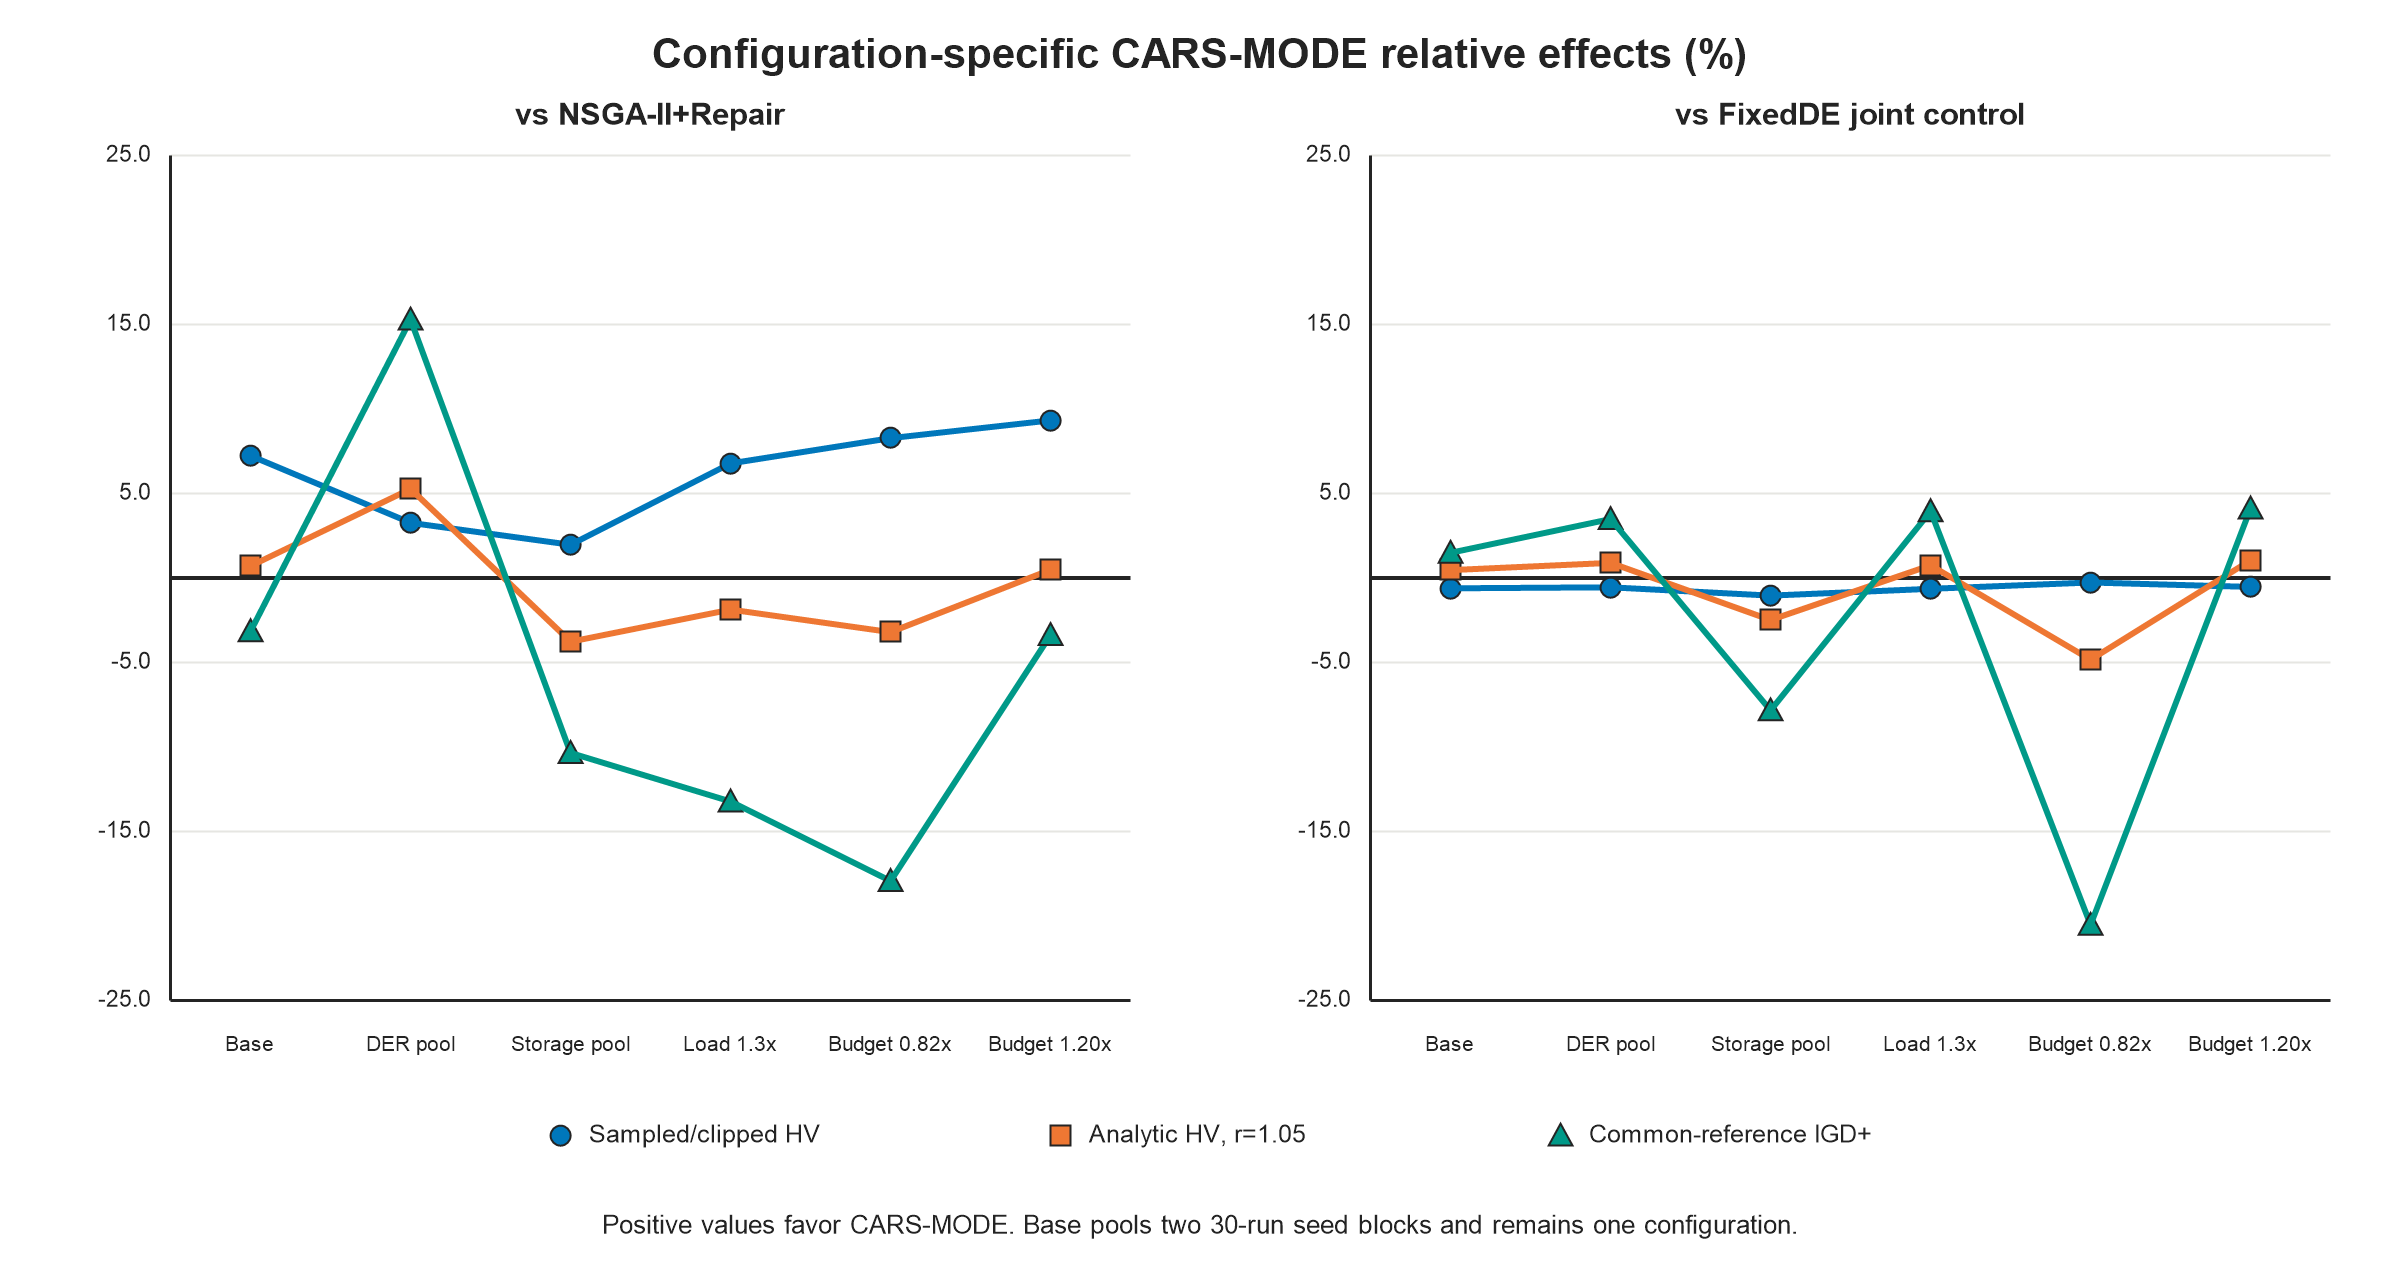
\includegraphics[width=0.94\textwidth]{figures/fig_configuration_effects.png}
\caption{Configuration-specific descriptive effects for sampled-bound/clipped HV, analytic HV at reference 1.05, and common-reference IGD+. Positive values favor CARS-MODE for all three series. The base point pools two independent 30-run seed blocks but remains one configuration; no confidence interval is implied by the connected points.}\label{fig:2}
\end{figure*}

\begin{table*}[t]
\centering
\footnotesize
\setlength{\tabcolsep}{3pt}
\caption{Equal-configuration descriptive summary for the proposed method and closest controls. Each of the six configurations receives one weight. HV is higher-is-better; IGD+ is lower-is-better.}\label{tab:6}
\begin{tabularx}{\textwidth}{@{}>{\raggedright\arraybackslash}X >{\raggedright\arraybackslash}X >{\raggedright\arraybackslash}X >{\raggedright\arraybackslash}X >{\raggedright\arraybackslash}X@{}}
\toprule
Method & Role & Sampled/clipped HV & Analytic HV, $r=1.05$ & Common-ref IGD+ \\
\midrule
Ablation-FixedDE & joint control & 0.04265615 & 0.00043690 & 0.02189851 \\
\textbf{CARS-MODE} & \textbf{proposed} & \textbf{0.04240014} & \textbf{0.00043464} & \textbf{0.02218917} \\
NSGA-II+Repair & external control & 0.03997622 & 0.00043530 & 0.02117209 \\
GDE3 & direct DE control & 0.03916542 & 0.00042639 & 0.02271159 \\
NSDE & direct DE control & 0.03913725 & 0.00042185 & 0.02366336 \\
\bottomrule
\end{tabularx}
\end{table*}

The complete 14-method table is generated as \texttt{derived\_tables/p3\_configuration\_weighted\_leaderboard.csv}. Under the archived legacy definition, CARS-MODE has a higher mean than each of eight stochastic baselines in all 56 seed-block cells spanning the six configurations; 55 differences remain significant after the original within-seed-block Holm correction. The unresolved cell is NSGA-II+Repair in \texttt{storage\_allocation}. Weighted Sum is lower in all seven descriptive seed-block comparisons and receives no seed-level p-value. These statements remain specific to the legacy metric. MOEA/D's penalty-based configuration collapses to the empty plan on this problem; that implementation-specific failure is not generalized to decomposition methods. Runtime from the validation rerun is retained as environment provenance and is not used to rank methods or claim engineering value.

\subsection{Ablation Study}\label{ablation-study}

Figure 3 compares the full method with the four controls/variants after first pooling the two base seed blocks and then giving equal weight to the six configurations.

\begin{figure*}[t]
\centering
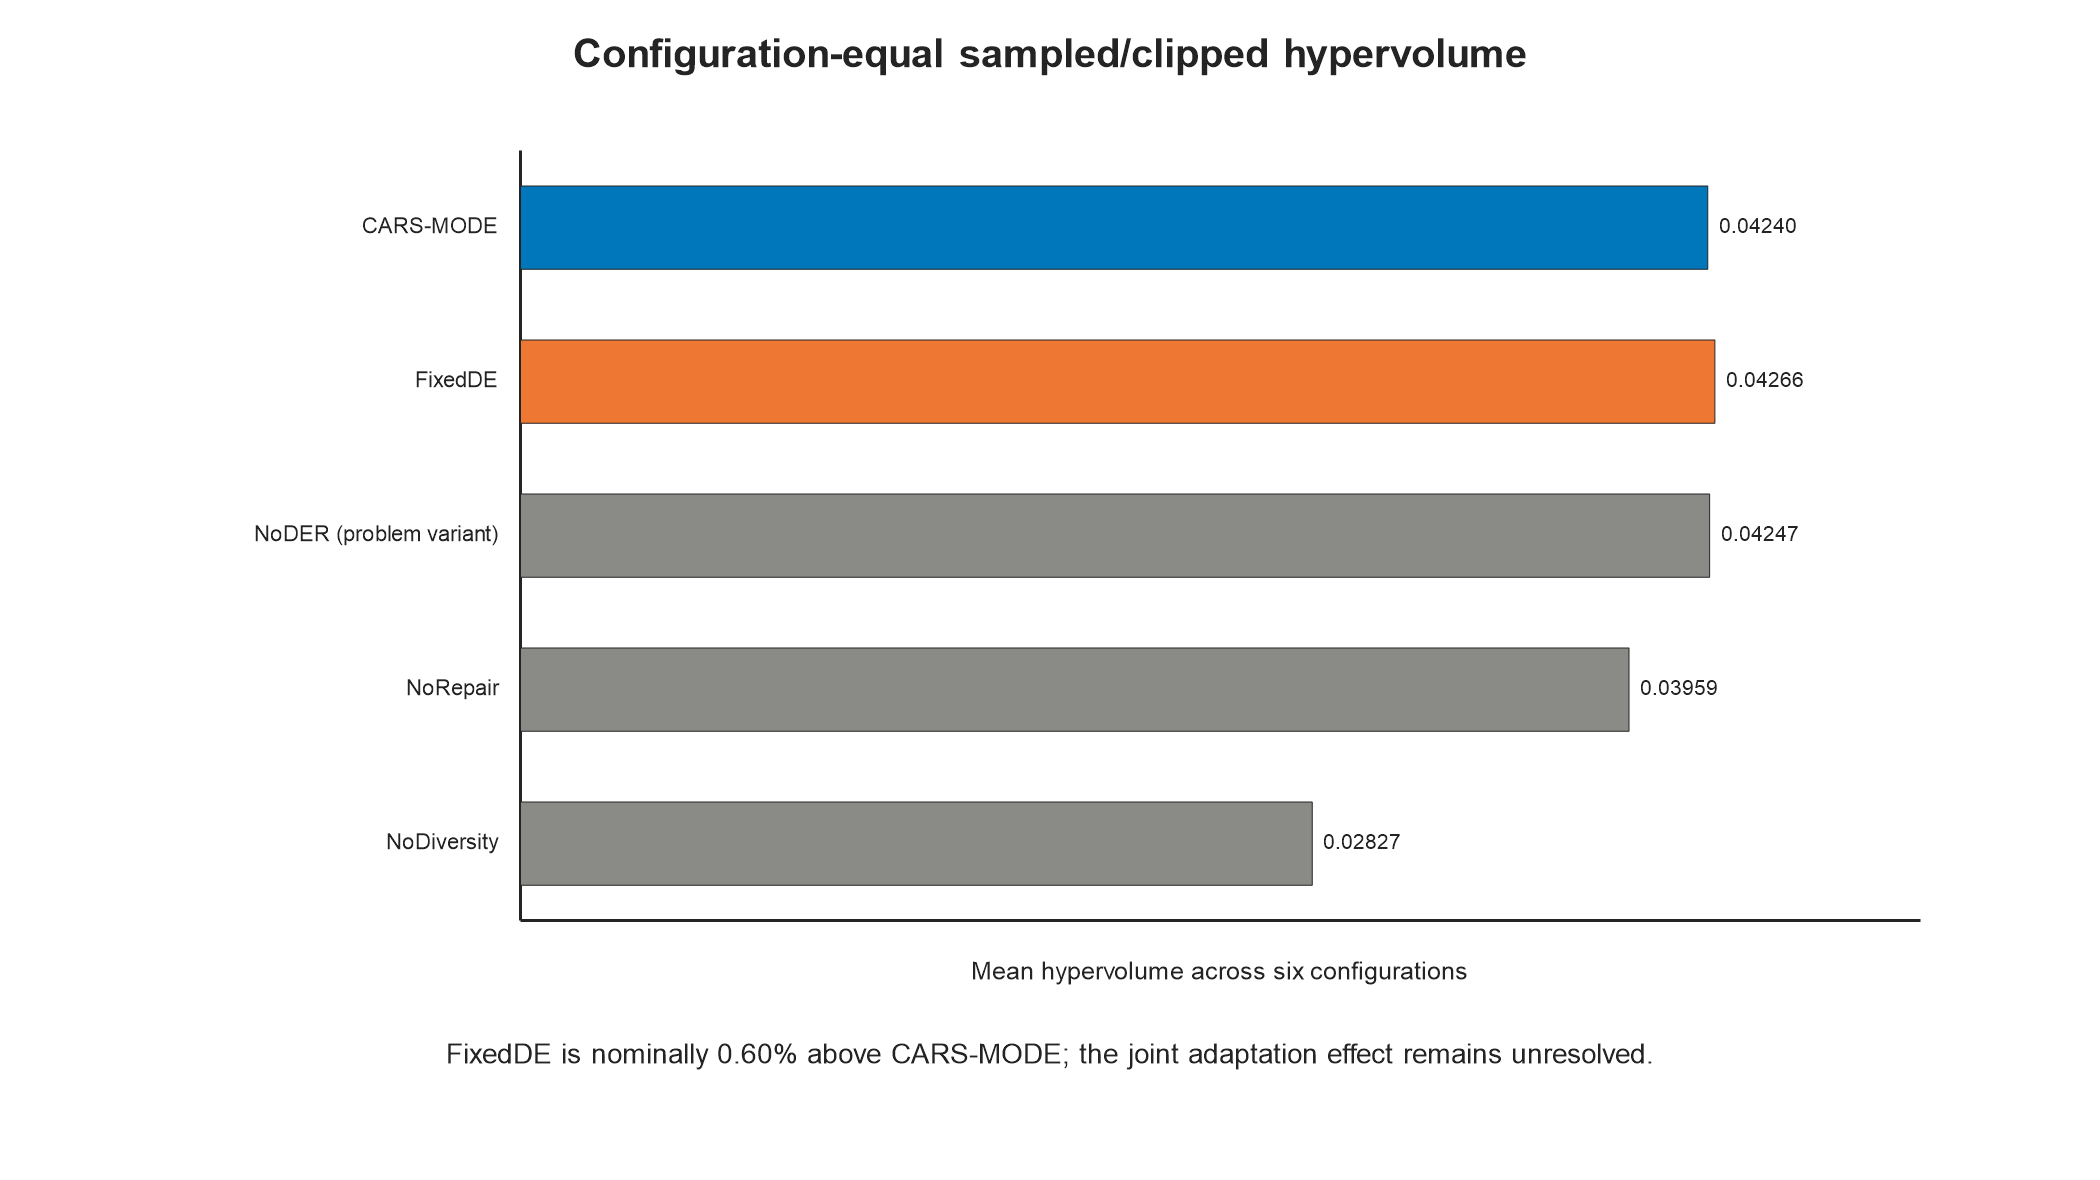
\includegraphics[width=0.94\textwidth]{figures/fig_ablation.png}
\caption{Equal-configuration sampled-bound/clipped hypervolume for CARS-MODE and four controls/variants. FixedDE is nominally higher and unresolved at the proxy level. NoDER changes the problem and is not a component ablation.}\label{fig:3}
\end{figure*}

Within sampled-bound/clipped HV, the combined controls support joint repair and diversity conclusions. Removing budget repair costs 6.63\% of the equal-configuration mean. It is significant in 6/7 seed blocks under the primary within-block opponent families and in 7/7 under the supplementary repair-specific Holm family. Removing crowding diversity costs 33.32\% and is significant in all seven seed blocks under both families, while the configuration-equal mean front size falls from 38.6 to 8.0. The FixedDE contrast is unresolved in all seven seed blocks under both families. The inferential counts retain both base seed blocks rather than pretending that they are separate problem configurations. Section 6.7 shows that the broad NoDiversity loss persists descriptively under analytic normalization, but the study does not claim that every component contrast is invariant to the metric.

\textbf{The combined adaptation bundle does not improve the legacy proxy indicator.} Ablation-FixedDE fixes \(F = 0.5\) and \(CR = 0.9\) and replaces the two-strategy pool with rand/1. It attains an equal-configuration mean of 0.04266, \textbf{0.60\% above the full method}. The difference is not Holm-significant in any of the seven seed blocks (adjusted p = 0.22--0.76, all nominally favoring FixedDE). Because this control changes parameter adaptation and strategy selection together, it does not identify their individual effects. Ablation-NoDER is similarly close (+0.16\%): the full method loses significantly in the tight-budget and DER-siting seed blocks and wins significantly in the loose-budget block. NoDER changes the candidate pool rather than an algorithmic component and is not used for component attribution. The FixedDE result does not support retaining the adaptive bundle for proxy accuracy; Section 6.3 treats the AC observations only as an illustrative secondary contrast.

\subsection{AC Load-Flow Validation and the HV--AC Trade-Off}\label{ac-load-flow-validation-and-the-hvac-trade-off}

Table 7 and Figure 4 report the archived pandapower diagnostic for each method present in that panel over 72 AC cases. GDE3, NSDE, and NSGA-II+Repair were not evaluated in the archived AC panel.

\begin{table*}[t]
\centering
\scriptsize
\setlength{\tabcolsep}{3pt}
\caption{Archived run-index-0 composition diagnostic. Stress-only excludes the base operating case (60 cases). Rows are dependent fixed-case evaluations, not optimizer-seed replications.}\label{tab:7}
\begin{tabularx}{\textwidth}{@{}>{\raggedright\arraybackslash}X >{\raggedright\arraybackslash}X >{\raggedright\arraybackslash}X >{\raggedright\arraybackslash}X >{\raggedright\arraybackslash}X >{\raggedright\arraybackslash}X@{}}
\toprule
Method & Role & AC-feasible rate & Stress-only rate & Mean min voltage (pu) & Mean max line loading (\%) \\
\midrule
No-Plan & reference & 0.500 & 0.400 & 0.9619 & 90.8 \\
Standard DE & baseline & 0.681 & 0.617 & 0.9731 & 63.5 \\
NSGA-II & baseline & 0.667 & 0.600 & 0.9739 & 75.6 \\
Ablation-NoRepair & ablation & 0.667 & 0.600 & 0.9735 & 70.5 \\
Ablation-NoDER & ablation & 0.667 & 0.600 & 0.9697 & 56.8 \\
GA & baseline & 0.639 & 0.567 & 0.9720 & 66.7 \\
\textbf{CARS-MODE} & \textbf{proposed} & \textbf{0.611} & \textbf{0.567} & \textbf{0.9729} & \textbf{76.6} \\
PSO & baseline & 0.611 & 0.533 & 0.9716 & 75.7 \\
Ablation-FixedDE & ablation & 0.569 & 0.517 & 0.9720 & 73.7 \\
Ablation-NoDiversity & ablation & 0.569 & 0.483 & 0.9681 & 69.9 \\
MOEA/D & baseline & 0.500 & 0.400 & 0.9619 & 90.8 \\
Weighted Sum & baseline & 0.500 & 0.400 & 0.9636 & 88.4 \\
\bottomrule
\end{tabularx}
\end{table*}
\begin{figure*}[t]
\centering
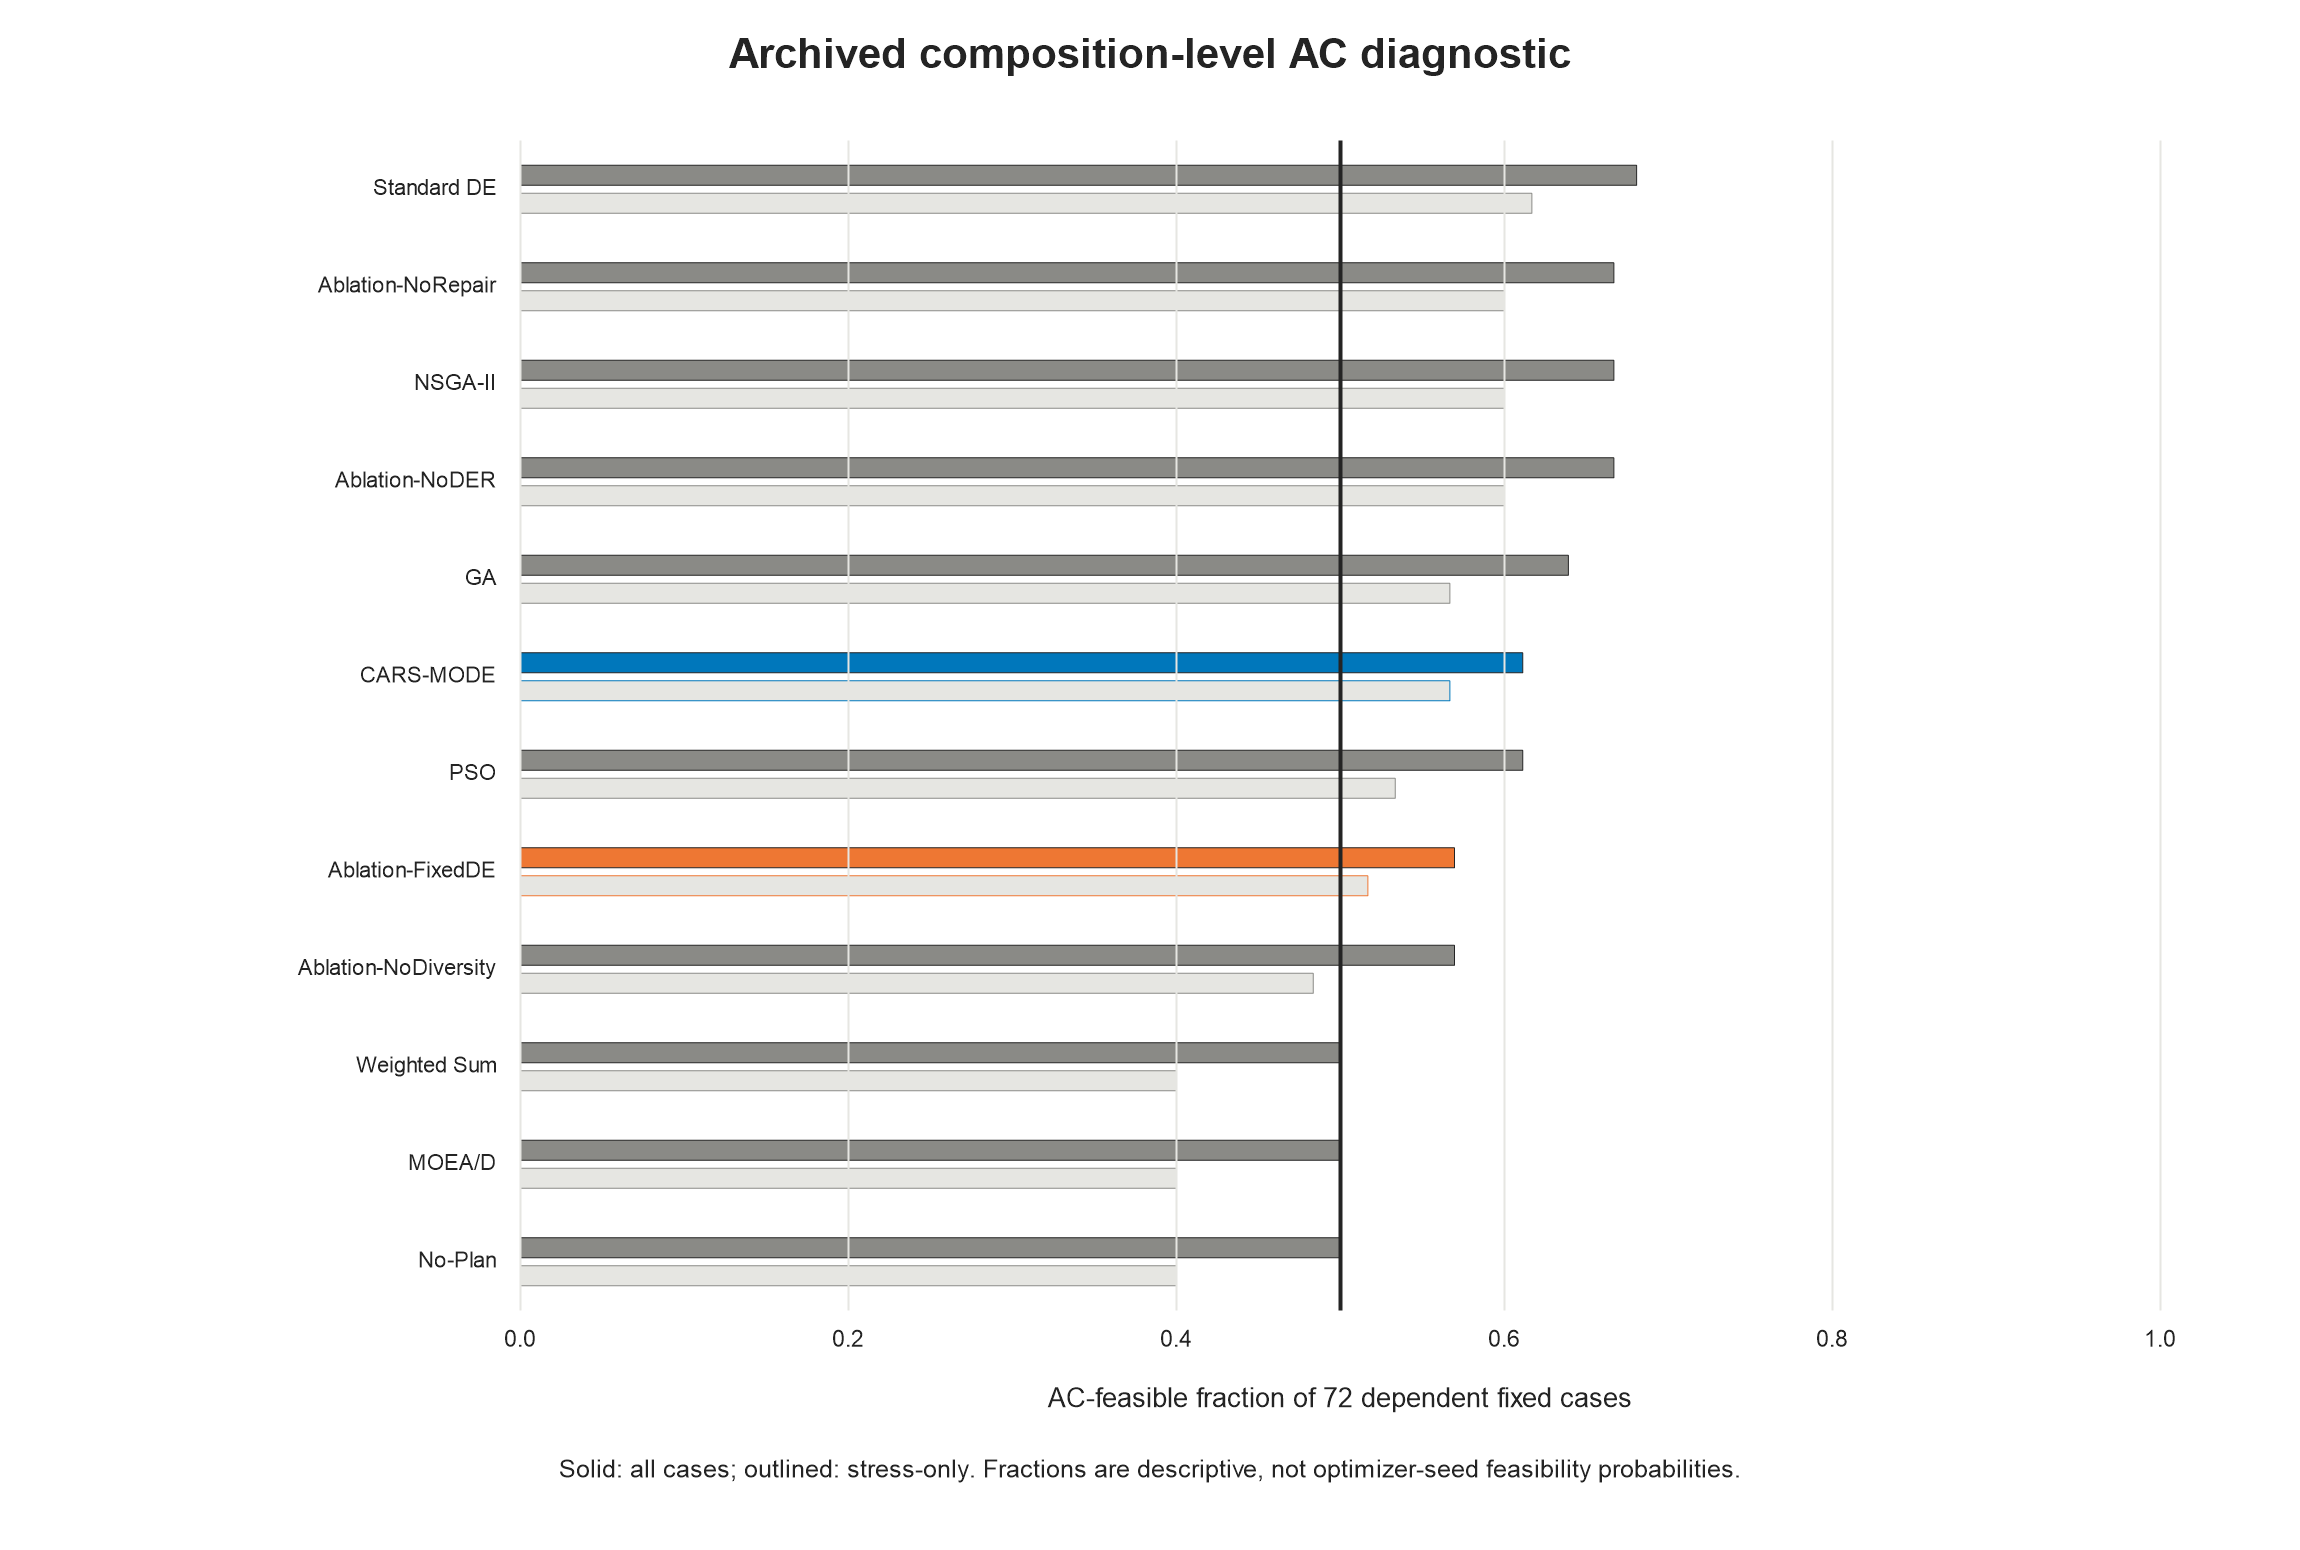
\includegraphics[width=0.94\textwidth]{figures/fig_ac_validation.png}
\caption{AC-feasible rate (all operating cases, upper bar; stress-only, lower bar) per method over 72 pandapower cases on four SimBench MV networks. The dashed line is the No-Plan reference (0.50).}\label{fig:4}
\end{figure*}

Three readings, in decreasing order of comfort for the proposed method.

First, most non-empty compromise plans improve the displayed AC diagnostics relative to the No-Plan reference. For CARS-MODE, the feasible rate is 0.611 versus 0.500 overall and 0.567 versus 0.400 under stress; the worst-bus voltage rises from 0.9619 to 0.9729 pu, and peak line loading falls from 90.8\% to 76.6\%. In the row-matched common panel, CARS-MODE changes 11 cases from infeasible to feasible and 3 in the reverse direction (net +8 of 72); its median changes relative to No-Plan are -16.97 percentage points in maximum line loading, -0.00068 pu in voltage violation, and -0.0752 MW in loss. These are descriptive paired changes without a seed-level or hierarchical interval. MOEA/D returns the empty plan and is therefore identical to No-Plan, while the automation-dominated Weighted Sum plan remains at the reference feasible rate of 0.500.

Second, \textbf{the proxy-hypervolume ranking does not transfer to the AC ranking.} CARS-MODE is mid-pack in the composition-level check: Standard DE reaches 0.681 AC feasibility, NSGA-II 0.667, GA 0.639, and CARS-MODE 0.611. The seed-0 CARS-MODE compromise contains 6 reinforcement, 7 storage, 1 DER, and 0 automation actions, whereas NSGA-II contains 5/4/6/0 and Standard DE 7/4/2/0. Under the common deterministic mapping, storage-rich compositions coincide with rural over-voltage and less reinforcement in urban growth cases. This is a descriptive composition pattern, not nodal causality or a randomized component effect. In storage\_allocation, CARS-MODE and NSGA-II have the same 8-reinforcement/5-storage composition, so 24 of their 72 AC cases coincide by construction. The 6.22\% equal-configuration legacy-HV margin over plain NSGA-II (6.06\% over NSGA-II+Repair) therefore provides no guarantee of AC-rank transfer.

Third, the AC inspection changes the interpretation of the joint-controller control. \textbf{Ablation-FixedDE, the nominal proxy winner (+0.60\%, n.s.), has an overall AC-feasible rate of 0.569 versus 0.611 for the full method} (stress-only 0.517 versus 0.567). Under stress-only operating cases, Ablation-NoDiversity is lower still (0.483). In the base-primary seed block, FixedDE selects eight storage actions compared with seven for CARS-MODE, and the additional mapped injection coincides with greater rural-network over-voltage. Conversely, NoRepair loses 6.63\% equal-configuration legacy hypervolume yet matches NSGA-II's AC rate of 0.667. These observations show that proxy and AC assessments capture different properties. Because the AC stage contains one run-index-0 compromise per method and selected seed block (72 dependent binary outcomes per method), it supports only a qualitative hypothesis about the \textbf{joint adaptation bundle}, not a statistically powered component claim (Section 8).

In the high-DER stress case, the No-Plan reference has an AC-feasible rate of 0.25, exceeding NSGA-II, PSO, and Ablation-NoRepair (all 0). This pattern is a \textbf{mapping-rule artifact}, not evidence that no planning is preferable. The AC validation sets DER injection proportional to the number of DER actions and applies a 2.5x DER factor at 0.5x load. Plans with more DER actions therefore inject more PV and incur more voltage violations. CARS-MODE contains one DER action, whereas NSGA-II contains six and produces severe over-voltage under this mapping. This regularity is a limitation of the composition-level validation (Section 8).

\subsection{Parameter Sensitivity Analysis}\label{parameter-sensitivity-analysis}

Parameter sensitivity is evaluated on the base proxy configuration with 10 seeds per point. Population size is varied as \(N_p\in\{20,40,60\}\), with NSGA-II re-run at each matched size. The jDE resampling probability is varied as \(\tau\in\{0.05,0.1,0.2\}\) against the default-population NSGA-II reference. The remaining mechanisms are binary switches covered by the ablation study. Table 8 and Figure 5 summarize the sweep.

\begin{table*}[t]
\centering
\footnotesize
\setlength{\tabcolsep}{3pt}
\caption{Exploratory parameter sensitivity on the base proxy configuration (10 seeds per point; nominal, multiplicity-unadjusted two-sided Mann--Whitney p-values versus the matched NSGA-II reference). The "$N_p$ = 40" and "$\tau$ = 0.1" rows are independent reruns of the same default configuration on different seed streams.}\label{tab:8}
\begin{tabularx}{\textwidth}{@{}>{\raggedright\arraybackslash}X >{\raggedright\arraybackslash}X >{\raggedright\arraybackslash}X >{\raggedright\arraybackslash}X >{\raggedright\arraybackslash}X@{}}
\toprule
Parameter & Value & CARS-MODE HV (mean +/- std) & NSGA-II reference & p (MWU) \\
\midrule
population size $N_p$ & 20 & 0.0382 +/- 0.0018 & 0.0329 & 0.0010 \\
population size $N_p$ & 40 (default) & 0.0409 +/- 0.0016 & 0.0385 & 0.0058 \\
population size $N_p$ & 60 & 0.0425 +/- 0.0007 & 0.0399 & 0.0002 \\
resampling prob. $\tau$ & 0.05 & 0.0407 +/- 0.0008 & 0.0385 & 0.0006 \\
resampling prob. $\tau$ & 0.1 (default) & 0.0410 +/- 0.0016 & 0.0385 & 0.0036 \\
resampling prob. $\tau$ & 0.2 & 0.0416 +/- 0.0011 & 0.0385 & 0.0002 \\
\bottomrule
\end{tabularx}
\end{table*}
\begin{figure*}[t]
\centering
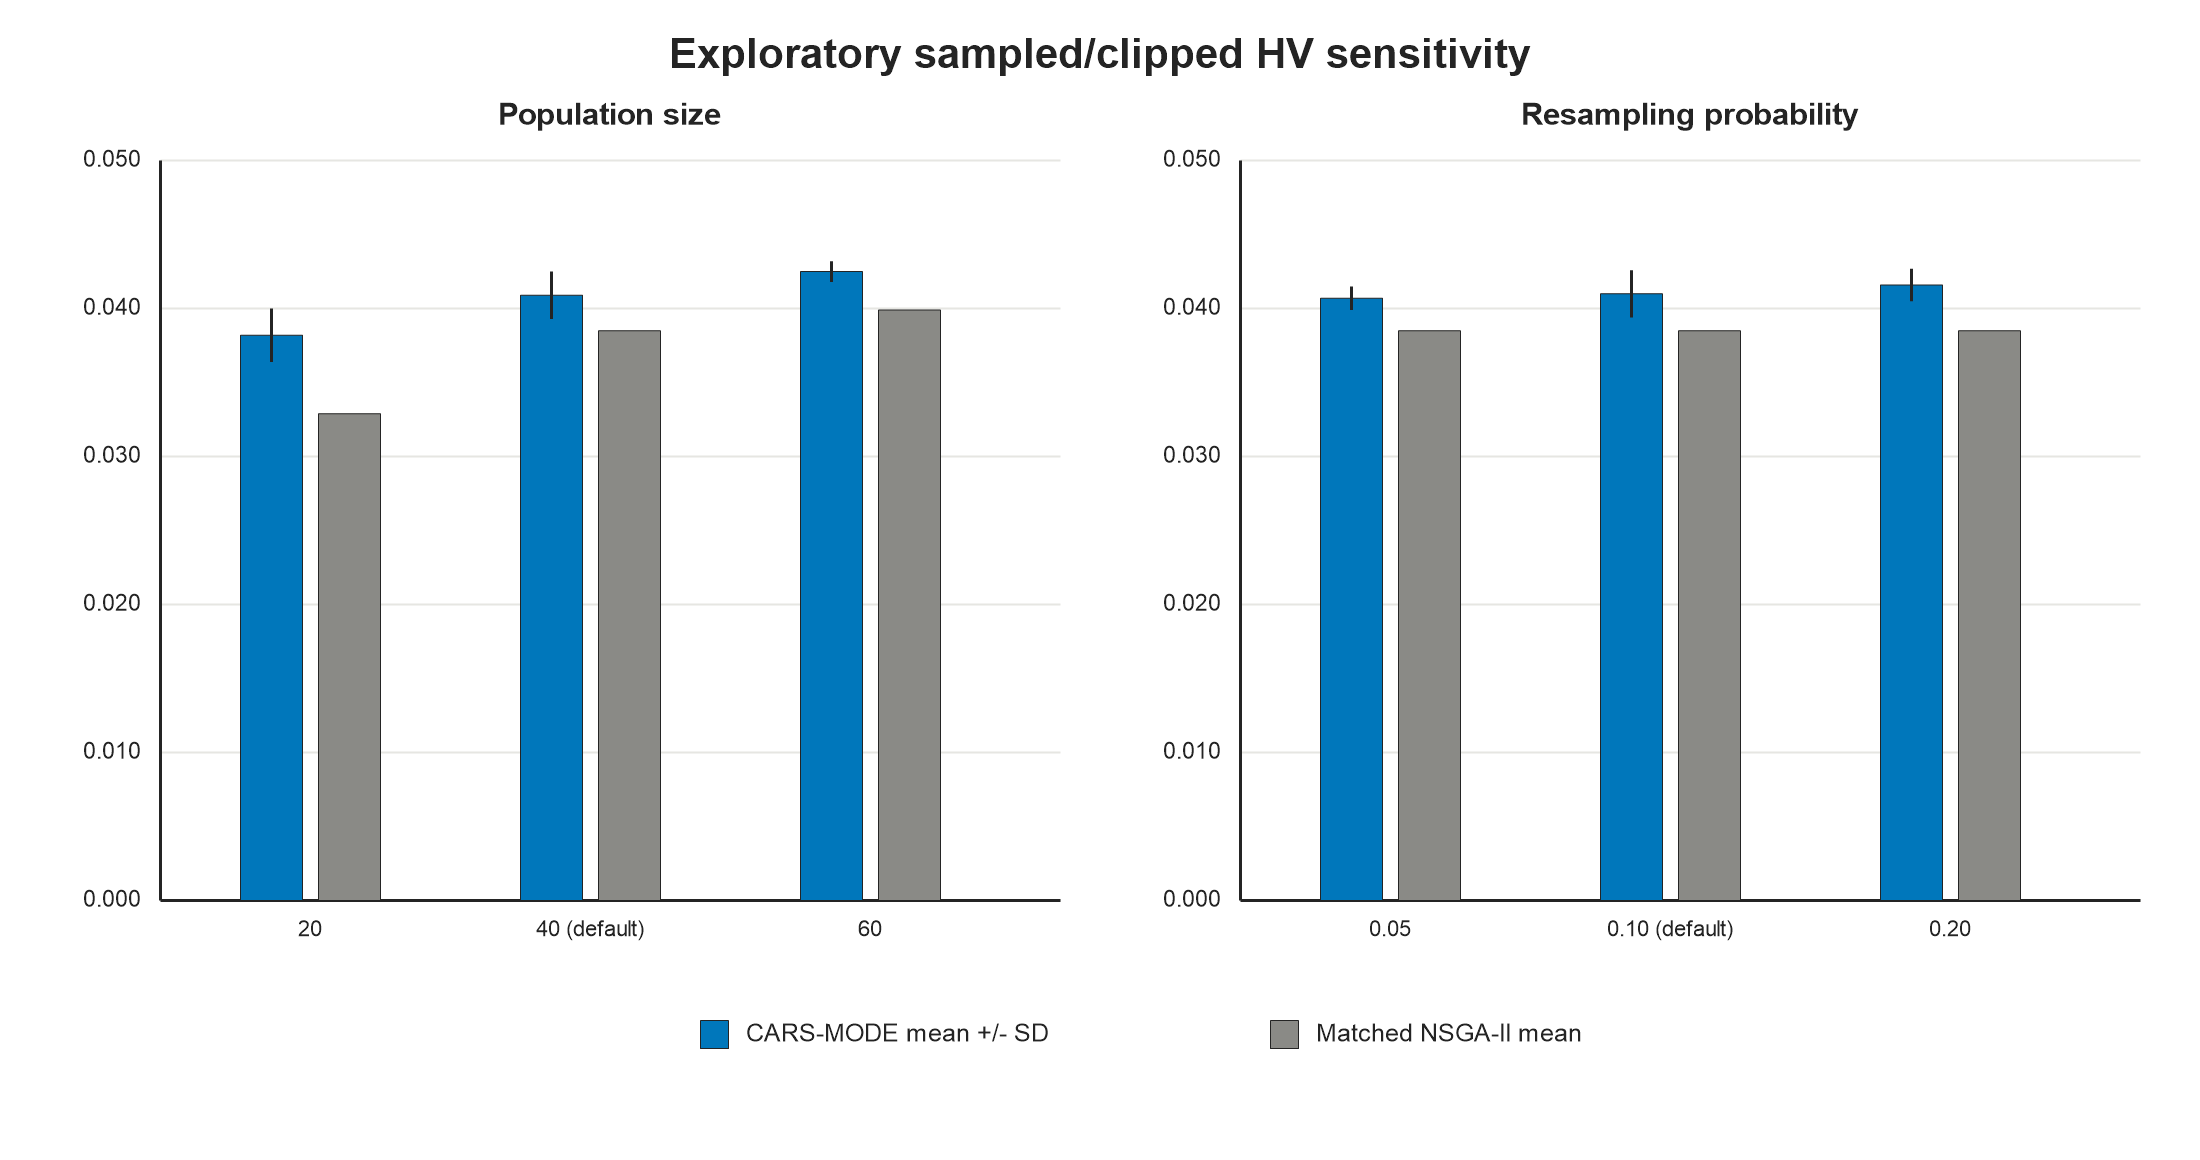
\includegraphics[width=0.94\textwidth]{figures/fig_sensitivity.png}
\caption{Mean hypervolume (+/- std over 10 seeds) of CARS-MODE across the population-size axis (\textbf{a}, NSGA-II re-run at matched sizes) and the jDE resampling-probability axis (\textbf{b}, NSGA-II reference at the default population).}\label{fig:5}
\end{figure*}

At every swept point CARS-MODE's mean hypervolume is above the corresponding NSGA-II reference (smallest absolute margin 0.0022), so no mean-rank reversal appears in the tested range. The nominal p-values are shown for transparency but do not define a confirmatory family. The \(\tau\) axis has a 2.3\% spread and the \(N_p\) axis a 10.5\% spread. The defaults (\(N_p=40\), \(\tau=0.1\)) are not the best observed points, reducing concern that the displayed configuration was selected at a visible peak.

The proxy indicator and AC-feasibility results differ partly because the algorithms return different compromise compositions. Figure 6 summarizes all rerun seed compromises after pooling the base seed blocks and weighting the six configurations equally. It describes the optimizer output distribution, not the three run-index-0 compositions evaluated in the archived AC panel. CARS-MODE allocates more actions to storage than NSGA-II and fewer to reinforcement than FixedDE in this summary. The visualization motivates composition inspection, but it does not establish nodal electrical causality: placement is imposed later by a common deterministic mapping.

\begin{figure*}[t]
\centering
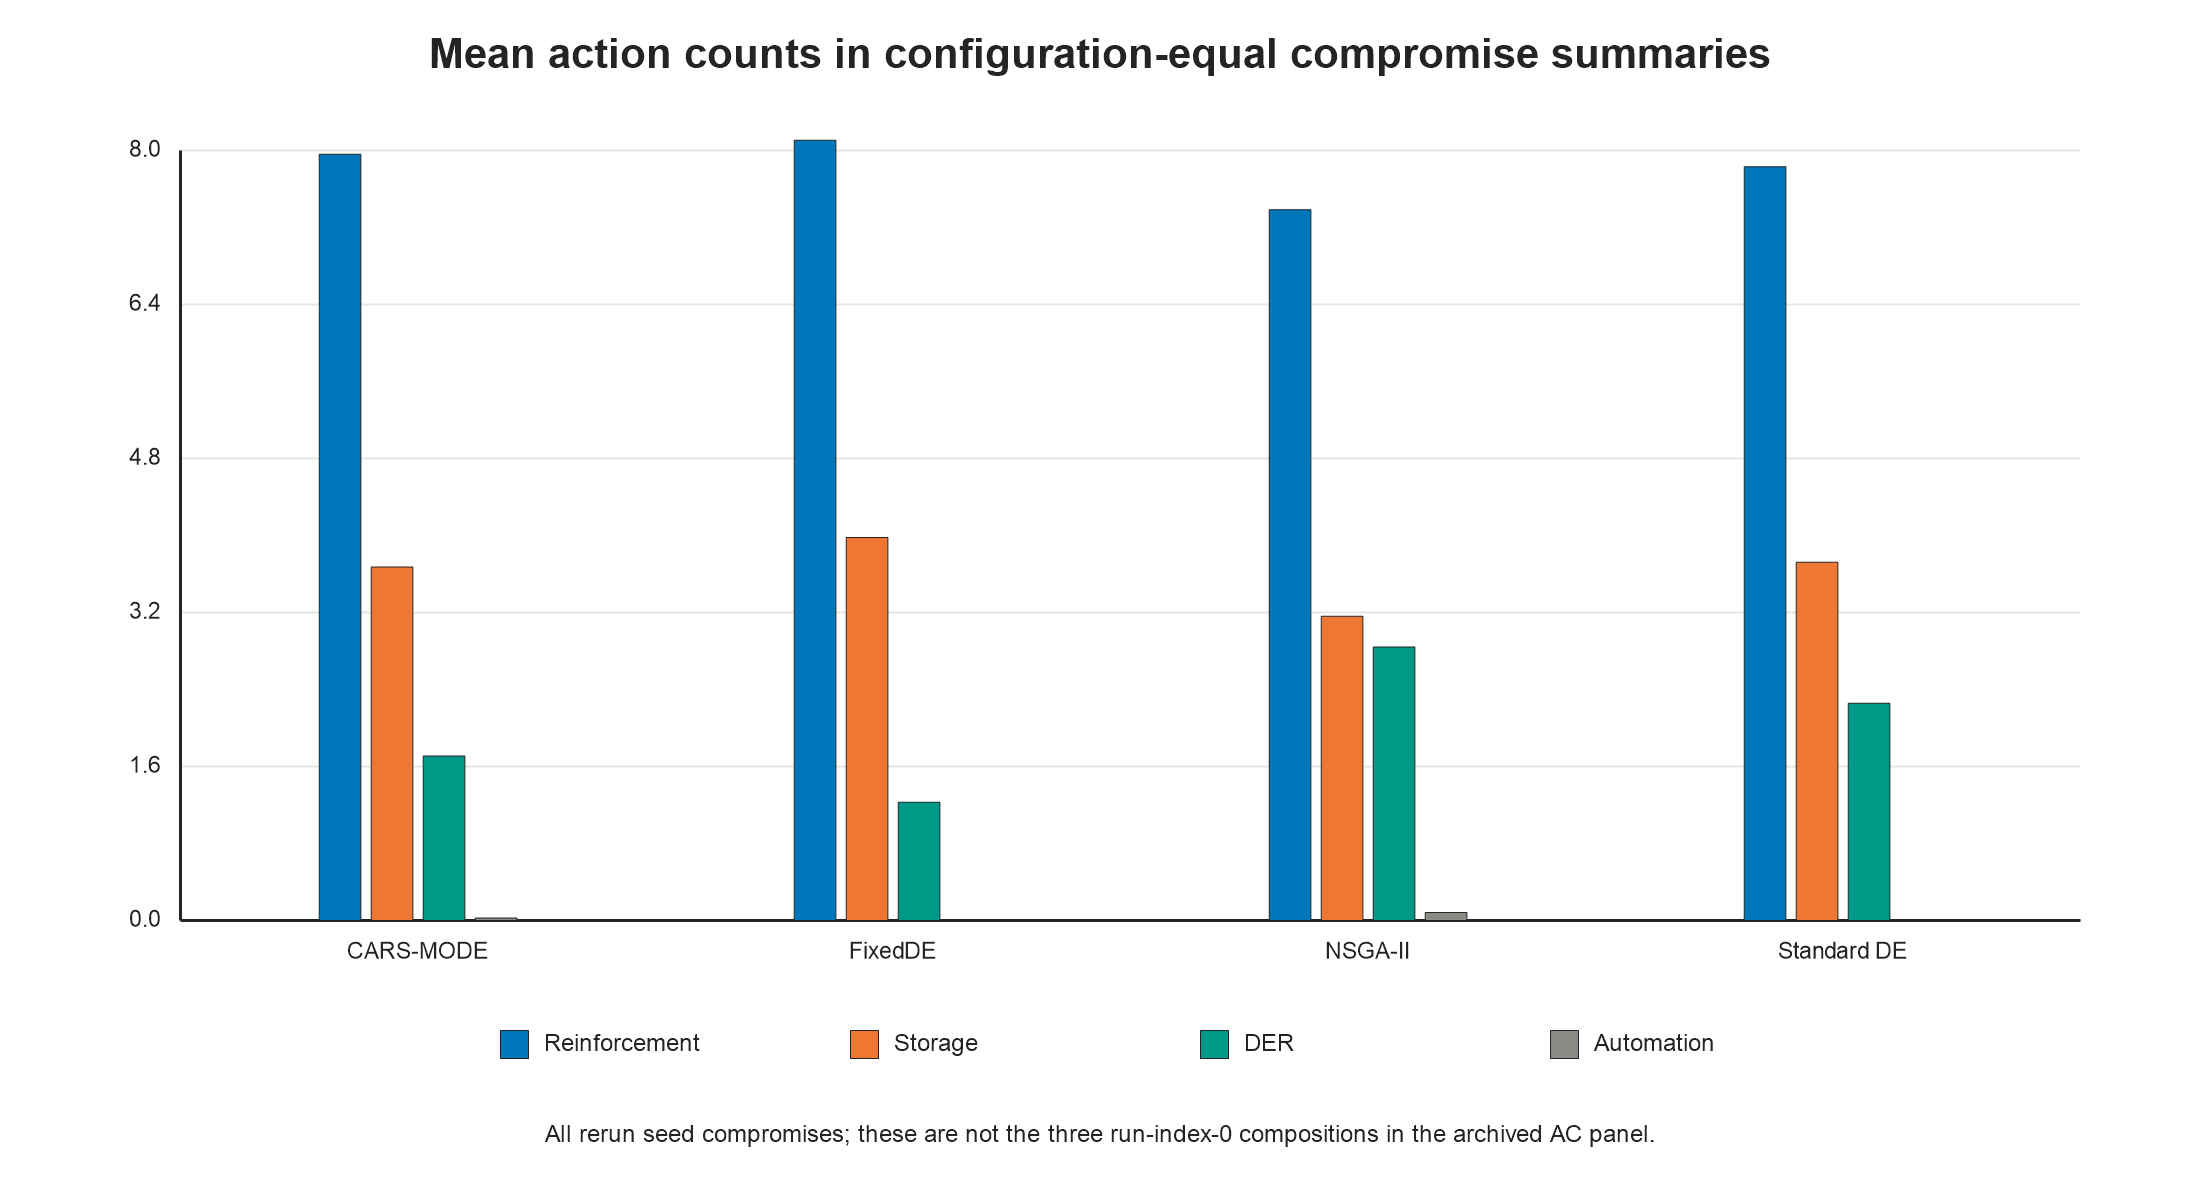
\includegraphics[width=0.94\textwidth]{figures/fig_portfolio_composition.png}
\caption{Mean number of reinforcement, storage, DER, and automation actions across all rerun seed compromises, with equal weight for six configurations and the two base seed blocks pooled first. These compromises were not evaluated by AC power flow. The bars identify portfolio differences before composition-to-network mapping and should not be interpreted as nodal siting decisions or AC-feasibility tests.}\label{fig:6}
\end{figure*}

\subsection{Configuration-Level Effects and Decision Value}\label{configuration-level-effects-and-decision-value}

The configuration effects in Table 5 change what can be used for a planning decision. The archived metric alone would select CARS-MODE over NSGA-II+Repair in every configuration, but analytic HV reverses that ordering in three configurations and common-reference IGD+ reverses it in five. FixedDE is 0.60\% higher on the equal-configuration legacy summary, 0.52\% higher on analytic HV at reference 1.05, and 1.31\% better on common-reference IGD+. Those small nominal differences do not establish an adaptation effect. They identify a shortlist whose ordering depends on the proxy diagnostic.

The engineering value supported by the AC layer is therefore \textbf{screening value}, not proof of physical feasibility. Figure 7 compares every archived method with the same No-Plan network/case rows. CARS-MODE changes 11 rows from infeasible to feasible and 3 in reverse (net +8), while its median maximum-loading change is -16.97 percentage points. FixedDE has net +5 and a larger median loading reduction (-22.75 points); Standard DE has net +13. These quantities answer whether a mapped composition merits further inspection. They do not estimate the probability that an optimizer or action portfolio is feasible because the 72 rows share only three run-index-0 compositions.

\begin{figure*}[t]
\centering
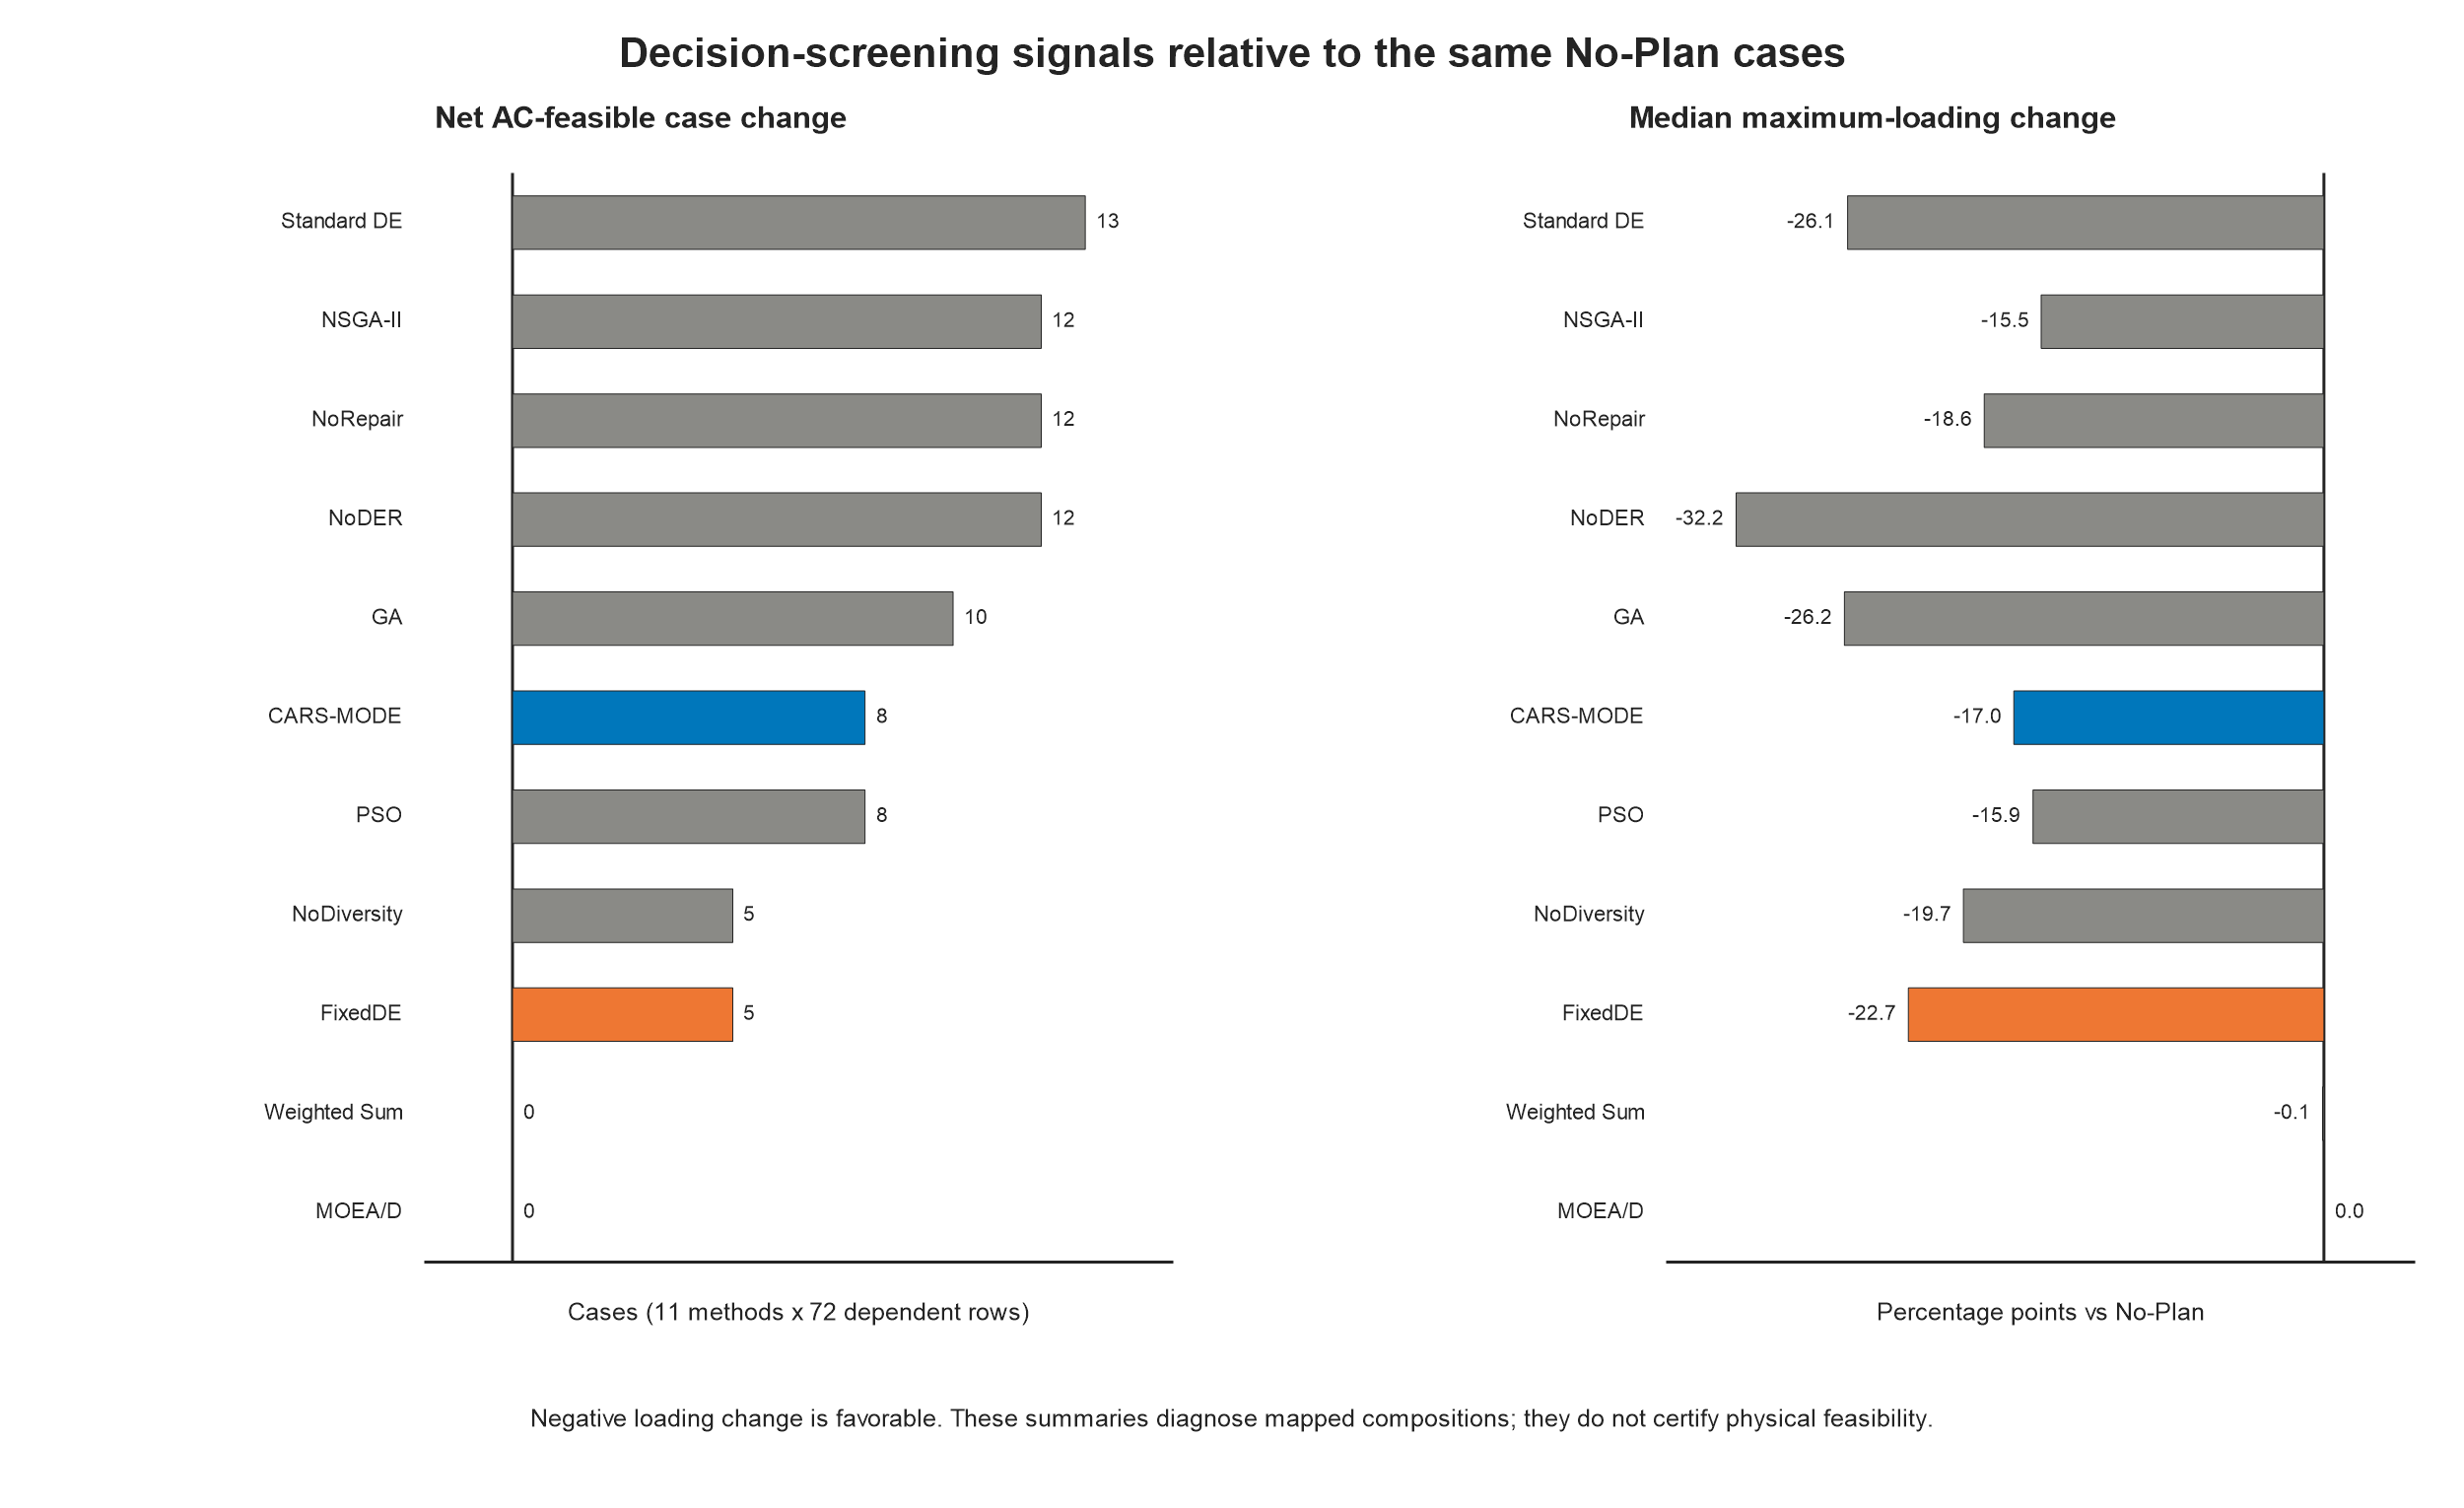
\includegraphics[width=0.94\textwidth]{figures/fig_decision_value.png}
\caption{Matched composition-level AC diagnostics relative to the same No-Plan rows. The left panel is the net count of infeasible-to-feasible minus feasible-to-infeasible transitions; the right panel is the median change in maximum line loading, where negative is favorable. All rows are dependent fixed-case evaluations from three mapped compositions per method. The figure does not report optimizer-seed physical feasibility.}\label{fig:7}
\end{figure*}

A pass/fail fraction also hides distance to the thermal boundary. Figure 8 displays the median and 95th percentile of maximum line loading over the same 72 cases. CARS-MODE has a median of 74.44\% and a 95th percentile of 134.36\%; NSGA-II is similar at 73.69\% and 128.09\%. NoDER has the lowest displayed values (53.88\% and 87.14\%), which reflects a different search problem and action mix rather than evidence that removing DER is generally preferable. Several methods cross 100\% in their upper tail even when their aggregate feasible fraction exceeds No-Plan.

\begin{figure*}[t]
\centering
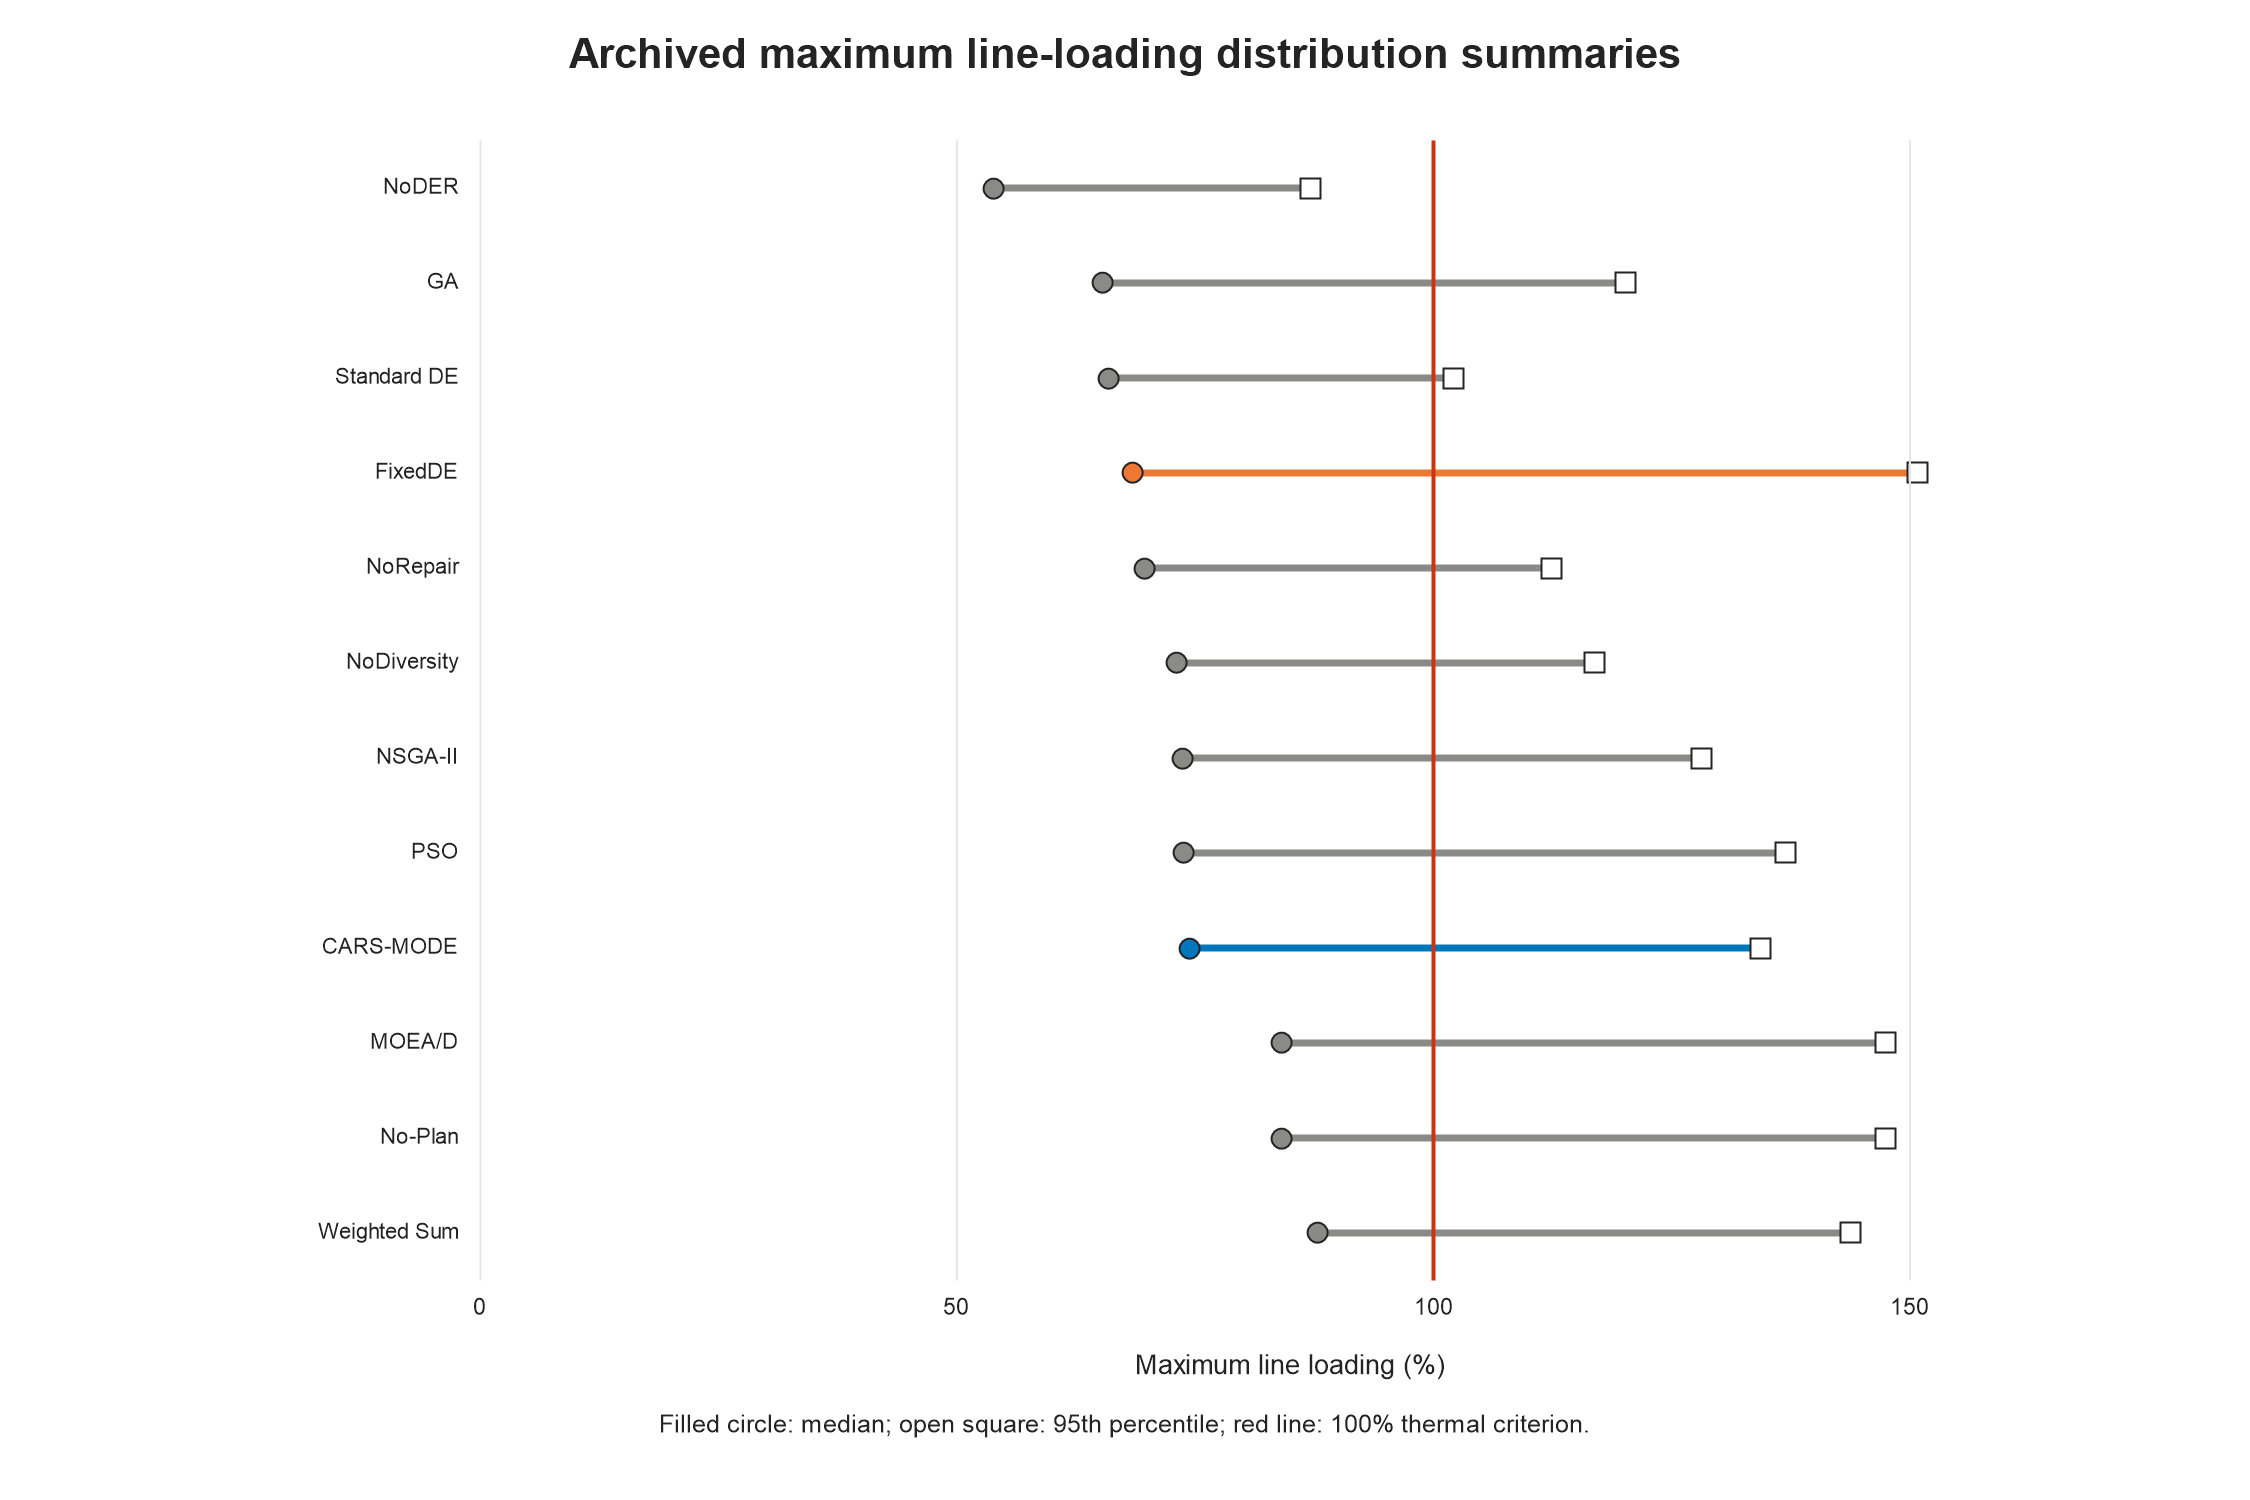
\includegraphics[width=0.94\textwidth]{figures/fig_ac_margin_distribution.png}
\caption{Median and 95th-percentile maximum line loading over the 72 pandapower validation cases per method. The red line marks the 100\% thermal criterion. The generated values are available in \texttt{derived\_tables/p3\_ac\_margin\_diagnostics.csv}.}\label{fig:8}
\end{figure*}

Together, Figures 7 and 8 define a defensible workflow: generate configuration-conditioned proxy fronts, retain more than one plausible method when rankings are diagnostic-sensitive, and apply physical checks to the shortlisted mapped actions. The current evidence supports that workflow but cannot certify action-aligned feasibility, monetary value, or deployment performance.

\subsection{Direct Multi-Objective DE Controls}\label{direct-multi-objective-de-controls}

GDE3 and NSDE close the most consequential gap in the original baseline set because both retain differential-evolution variation and Pareto-based environmental selection. Under configuration-equal sampled-bound/clipped HV, their values are 0.03917 and 0.03914, respectively, compared with 0.04240 for CARS-MODE. The corresponding relative margins are 8.26\% over GDE3 and 8.34\% over NSDE. CARS-MODE has a higher mean and a Holm-significant difference against both direct controls in all seven seed blocks spanning the six configurations (14 of 14 comparisons). Figure 9 reports six configuration means, pooling the two base seed blocks only within the base point. With analytic-bound HV, however, only one of seven seed-block comparisons is Holm-significant in CARS-MODE's favor against each direct control; common-reference IGD+ favors CARS-MODE by mean in four of seven seed blocks against each, again with one significant favorable contrast. The direct-control conclusion is therefore metric-specific.

\begin{figure*}[t]
\centering
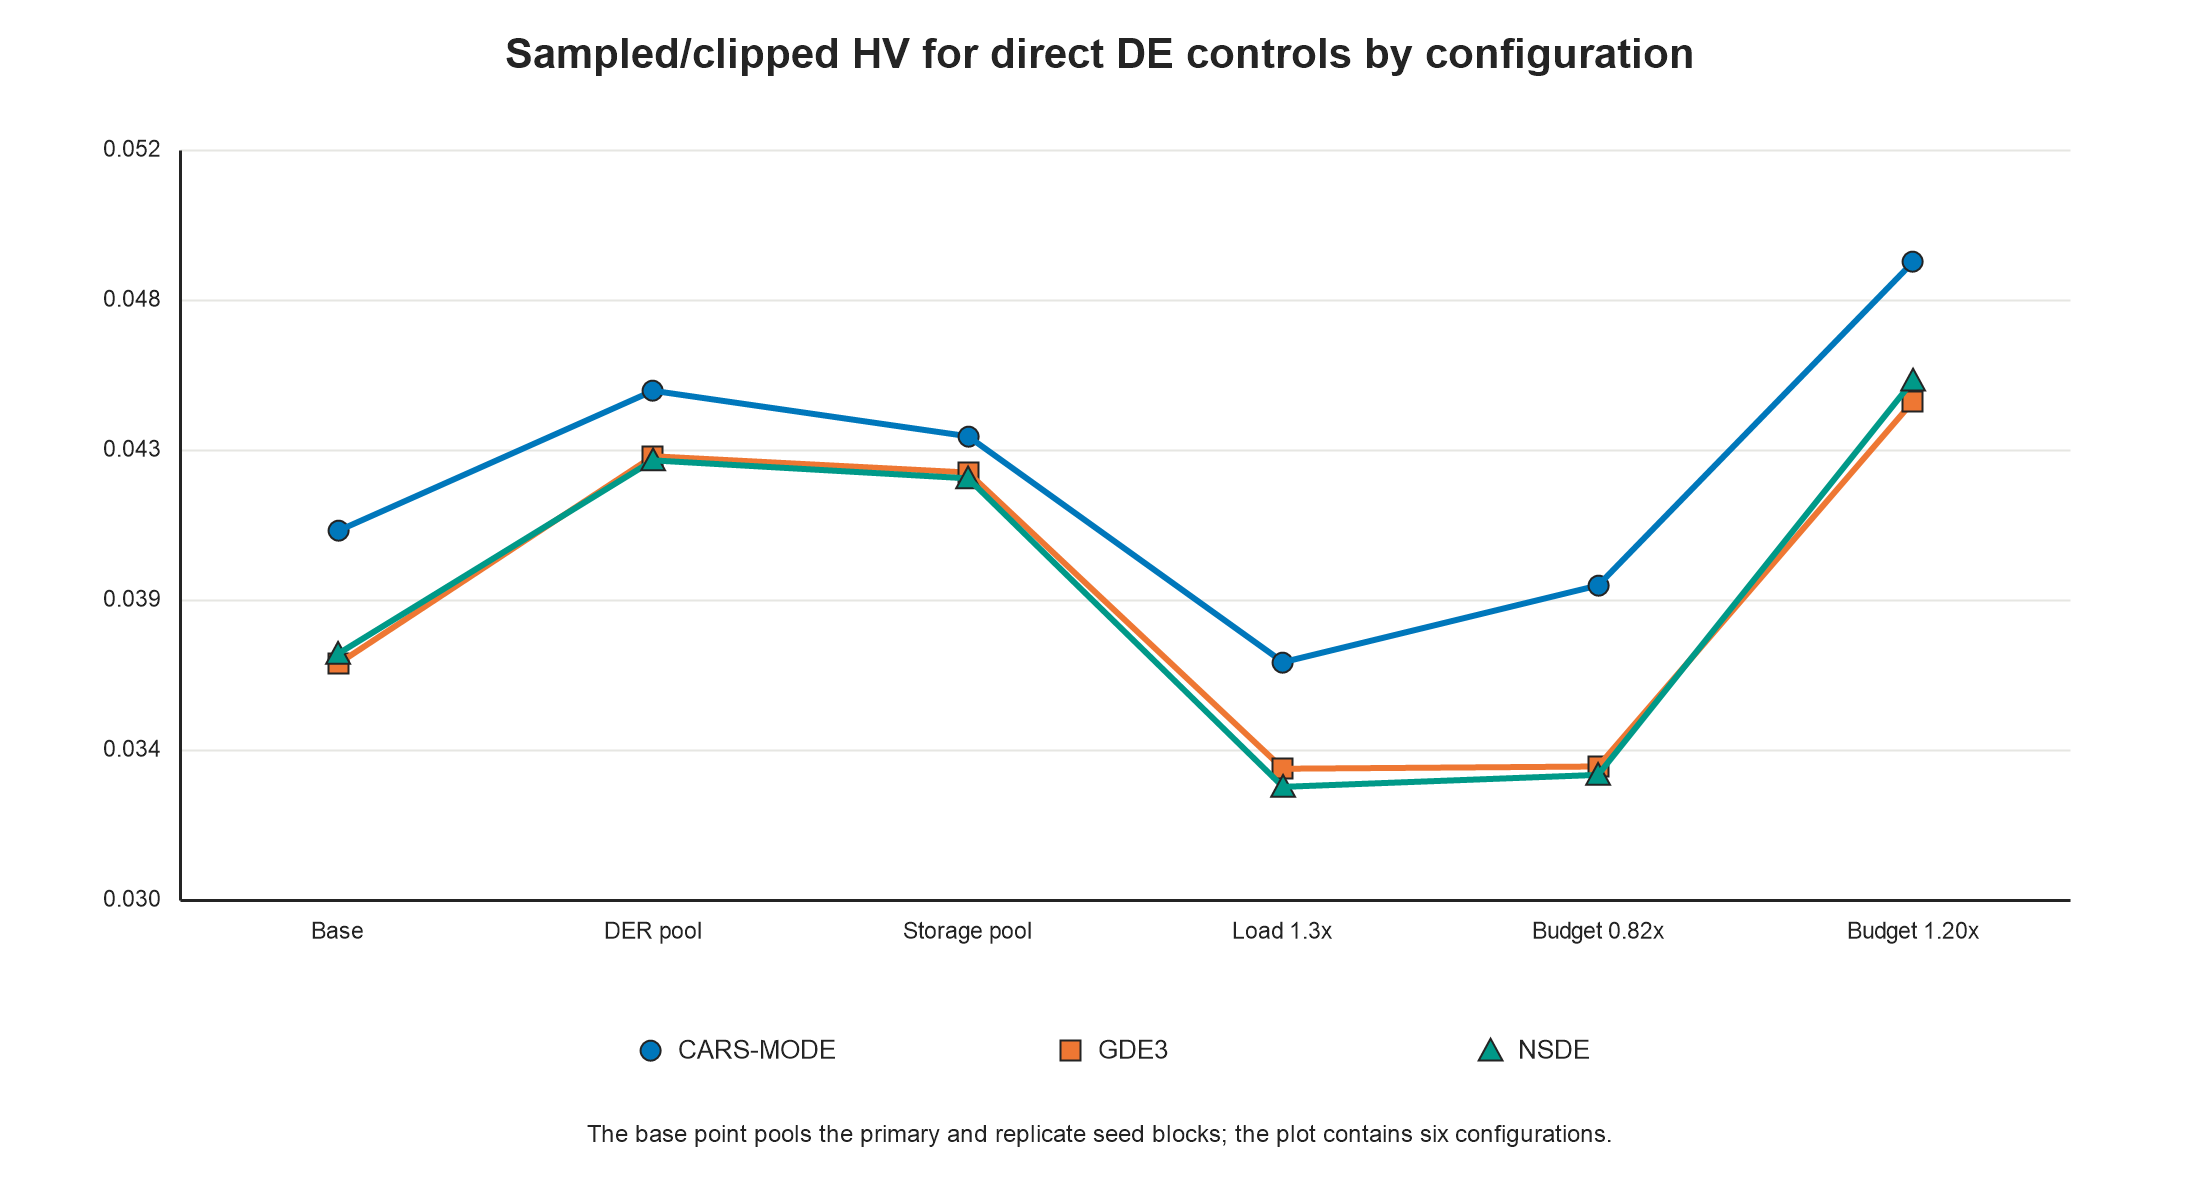
\includegraphics[width=0.94\textwidth]{figures/fig_direct_de_controls.png}
\caption{Mean sampled-bound/clipped hypervolume for CARS-MODE, GDE3, and NSDE in six configurations. The base point pools two independent 30-run seed blocks; other points use 30 runs. All fourteen seed-block CARS-MODE-versus-control tests are significant after Holm correction for this legacy metric. The analytic-bound and common-reference diagnostics are less favorable, and the combined FixedDE control remains statistically inseparable from the full method.}\label{fig:9}
\end{figure*}

\subsection{Reference-Point, Clipping, and Common-Reference Diagnostics}\label{reference-point-clipping-and-common-reference-diagnostics}

The exact rerun exposes a material property of the archived normalization. Among 68,248 returned front points, 2189 points contain at least one sampled-normalized coordinate below zero, for 2281 clipped coordinates in total: 1750 voltage-risk and 531 negative-reliability coordinates. No coordinate exceeds one. Before clipping, the 1.10 reference strictly dominates every point, with a minimum coordinate-wise margin of 0.14545. Clipping is therefore unnecessary for reference dominance here; it floors improvements beyond the sampled lower envelope and can change relative dominated volumes.

\begin{table*}[t]
\centering
\scriptsize
\setlength{\tabcolsep}{3pt}
\caption{Configuration-equal robustness diagnostics. HV is higher-is-better; IGD+ is lower-is-better. Ranks give each of six configurations one weight. "Favorable configurations" uses configuration means; significance columns retain the seven upstream seed-block tests and their within-block Holm correction over twelve stochastic opponents.}\label{tab:9}
\begin{tabularx}{\textwidth}{@{}>{\raggedright\arraybackslash}X >{\raggedright\arraybackslash}X >{\raggedright\arraybackslash}X >{\raggedright\arraybackslash}X >{\raggedright\arraybackslash}X >{\raggedright\arraybackslash}X >{\raggedright\arraybackslash}X@{}}
\toprule
Metric & CARS-MODE & NSGA-II+Repair & CARS rank & Favorable configurations & Significant favorable seed blocks & Significant unfavorable seed blocks \\
\midrule
Sampled bounds, clipped HV, $r=1.10$ & 0.04240014 & 0.03997622 & 3 & 6/6 & 6/7 & 0/7 \\
Analytic bounds, HV, $r=1.10$ & 0.00212109 & 0.00213852 & 4 & 3/6 & 1/7 & 1/7 \\
Analytic bounds, HV, $r=1.05$ & 0.00043464 & 0.00043530 & 4 & 3/6 & 1/7 & 1/7 \\
Common-reference IGD+ & 0.02218917 & 0.02117209 & 5 & 1/6 & 1/7 & 0/7 \\
\bottomrule
\end{tabularx}
\end{table*}

The alternative 1.05 reference dominates every analytic-normalized point by at least 0.05. At that reference, NSGA-II+Repair is 0.15\% higher than CARS-MODE in the equal-configuration mean, and CARS-MODE ranks fourth behind the problem-variant NoDER, FixedDE, and NSGA-II+Repair. Common-reference IGD+ ranks CARS-MODE fifth, behind NoDER, NSGA-II+Repair, FixedDE, and plain NSGA-II. FixedDE's nominal advantage is retained under every equal-configuration summary: 0.60\% for legacy HV, 0.52\% for analytic HV at 1.05, and 1.31\% for IGD+. NoDER's first-place rank is not a component result because it changes the feasible decision pool. The empirical IGD+ reference contains the non-dominated union of all tested methods and seeds within each seed block and is therefore complementary, not independent. Collectively, these checks reject a normalization-invariant external-control advantage while retaining the narrower finding that CARS-MODE is competitive within the implemented constrained-search set.

\begin{center}\rule{0.5\linewidth}{0.5pt}\end{center}

\section{Discussion}\label{discussion}

\textbf{What the two-level evaluation supports.} CARS-MODE attains higher sampled-bound/clipped hypervolume than every external baseline tested in all six configurations, including NSGA-II with returned-population repair, GDE3, and NSDE. That ordering is not invariant: under analytic feasible envelopes, NSGA-II+Repair is 0.15\% higher at reference 1.05 in the equal-configuration summary, and common-reference IGD+ ranks CARS-MODE fifth. FixedDE is nominally higher on all three equal-configuration summaries and statistically unresolved in the pairwise analytic comparisons, so the evidence does not attribute a gain to adaptation. The archived AC layer shows that mapped compositions can improve some fixed-case diagnostics while also demonstrating that proxy rank does not determine electrical rank. It remains illustrative because neither multi-seed AC evaluation nor hierarchical optimizer uncertainty is available.

\textbf{Why the adaptive controller remains exploratory.} FixedDE is nominally 0.60\% higher on the archived legacy metric, 0.52\% higher on analytic HV at reference 1.05, and 1.31\% better on common-reference IGD+; none of the seven analytic-bound seed-block contrasts establishes a significant CARS-MODE advantage. The current joint control cannot determine whether one adaptive subcomponent helps while the other hurts. The AC inspection notes that FixedDE selects one additional storage action in the base-primary seed block (8 versus 7), and the mapped plan coincides with greater over-voltage in the rural network and less reinforcement in urban growth cases. This pattern is insufficient for a causal claim. More generally, proxy and external diagnostics can assign different apparent value to a mechanism group; the corresponding contrast for budget repair (6.63\% on equal-configuration legacy HV, AC-neutral in aggregate) reinforces the need to report both levels.

\textbf{Why the complete framework can be competitive without a resolved adaptation-bundle effect.} Removing diversity or repair reduces the effective set of feasible trade-off solutions on the archived metric, whereas jointly fixing the DE parameters and restricting mutation to rand/1 leaves that set almost unchanged. The GDE3 and NSDE comparisons place the complete constrained-search pipeline within a competitive multi-objective DE set, but their apparent margins shrink under analytic normalization and the FixedDE result prevents attribution to either adaptive subcomponent. Framework-level and component-level conclusions are therefore distinct; the combined ablations support only their declared joint contrasts.

\textbf{Practical reading for planners.} Front-returning methods provide trade-off sets and rank above the scalarized controls on each reported proxy diagnostic, but the illustrative AC composition check does not preserve that ordering; Standard DE has the highest mapped AC-feasible fraction. CARS-MODE's effect over NSGA-II+Repair is positive in every configuration only under the sampled-bound/clipped metric. A proxy front should therefore serve as a candidate-generation stage whose survivors undergo action-aligned power-flow checks. The supported decision value is the ability to expose configuration and diagnostic sensitivity before committing to that more expensive evaluation, not a claim that proxy stability implies physical feasibility.

\begin{center}\rule{0.5\linewidth}{0.5pt}\end{center}

\section{Limitations}\label{limitations}

We state the boundaries of this study explicitly.

\begin{enumerate}
\def\labelenumi{\arabic{enumi}.}
\tightlist
\item
  \textbf{Composition-level, not nodal, planning.} The optimizer selects subnet-level actions, and the AC validation maps plan \emph{compositions} onto concrete networks with fixed rules that choose buses by stress heuristics. Node-level siting and sizing---where method differentiation at the electrical layer would have to be demonstrated---is not performed, and the AC stage's per-method sample (72 dependent binary cases from one run-index-0 compromise in each of three selected seed blocks) supports qualitative patterns, not significance tests. Consequently, the high-DER case's No-Plan advantage is a mapping-rule artifact (Section 6.3) rather than a general electrical finding.
\item
  \textbf{Proxy objectives.} The five planning objectives are analytic indices of SimBench subnet statistics, not power-flow quantities; Section 6.3 measures, rather than assumes, their relation to AC feasibility, and finds it imperfect. Claims about ``planning quality'' in this paper mean proxy hypervolume unless explicitly stated otherwise.
\item
  \textbf{Normalization sensitivity.} Sampled lower bounds clip 2281 below-zero coordinates even though the 1.10 reference already dominates every un-clipped point. Analytic envelopes and common-reference IGD+ change the leading external-control order. The empirical IGD+ reference also contains the compared methods, so it is complementary rather than independent. No consistent-optimizer-superiority claim survives these diagnostics.
\item
  \textbf{Costs are not monetarily calibrated.} Candidate costs are synthetic cost units derived from network statistics. No engineering-economic conclusion (payback, deferral value) can be drawn before calibration against published utility investment figures.
\item
  \textbf{Single benchmark family.} All six planning configurations and the internal base replication derive from one SimBench network family. Standard distribution test systems (IEEE 33/69-bus) with nodal candidates are the natural second family and remain future work.
\item
  \textbf{Deterministic operating conditions.} Each planning configuration uses one fixed proxy operating point, and the AC layer uses six fixed operating/stress cases. Only optimizer initialization and variation are stochastic. A planning stage with sampled load/DER/outage scenarios would strengthen the robustness reading.
\item
  \textbf{Baseline configuration caveats.} MOEA/D's failure here is a failure of the specific penalty-based pymoo configuration on this problem; a tuned decomposition method might be competitive, and the comparison should not be quoted against MOEA/D generally. The archived configuration did not pin the pymoo version; the exact rerun used the preserved source with pymoo 0.6.2, but earlier library-default Boolean crossover/mutation probabilities cannot be certified independently of that reconstruction.
\item
  \textbf{The direct DE comparison is still bounded.} GDE3 and NSDE provide Pareto-based multi-objective DE controls under the same population and generation budget, but JADE-, SHADE-, and L-SHADE-derived multi-objective implementations remain absent. The evidence concerns the implemented configurations, not the entire adaptive-DE family.
\end{enumerate}

\begin{center}\rule{0.5\linewidth}{0.5pt}\end{center}

\section{Conclusions}\label{conclusions}

This study evaluates a constraint-aware, strategy-pool multi-objective DE on a SimBench-derived mixed-voltage portfolio proxy for distribution planning. It does not evaluate action-aligned, nodal expansion decisions. The exact 2940-run rerun comprises six distinct configurations plus an internal base replication. With equal configuration weight, CARS-MODE's sampled-bound/clipped hypervolume is 0.04240014, 6.06\% above NSGA-II with returned-population repair; the direct GDE3 and NSDE contrasts also favor it on that legacy metric. The audit finds 2281 below-zero clipped coordinates among 68,248 returned front points despite strict reference dominance before clipping.

Under unclipped analytic envelopes and reference 1.05, CARS-MODE scores 0.00043464 versus 0.00043530 for NSGA-II+Repair and ranks fourth; common-reference IGD+ ranks it fifth. FixedDE remains nominally ahead on every equal-configuration diagnostic, so the combined parameter-and-strategy adaptation bundle is unresolved. The repair and diversity ablations retain their scope as joint contrasts on the archived metric; NoDER remains a different problem rather than a component test.

The archived pandapower layer is an illustrative composition diagnostic: one run-index-0 compromise per method and selected seed block produces dependent fixed-case rows, not hierarchical optimizer uncertainty. CARS-MODE maps to 0.611 overall AC feasibility versus 0.500 for No-Plan and 0.667 for NSGA-II, with 11 matched infeasible-to-feasible transitions and 3 reversals relative to No-Plan. Those observations support a configuration-sensitive candidate-generation and physical-screening workflow, not electrical superiority or feasibility certification. Nodal siting, multi-seed AC mapping, monetary calibration, a second benchmark family, and separate adaptation controls remain necessary extensions.

\begin{center}\rule{0.5\linewidth}{0.5pt}\end{center}

\section*{Author Contributions}

{[}AUTHOR INPUT REQUIRED: assign the CRediT roles to Linyao Zhang, Jieyun Zheng, Zhanghuang Zhang, Shiyuan Ni, and Guilian Wu, and obtain approval from every author.{]} All authors have read and agreed to the published version of the manuscript.

\section*{Funding}

{[}AUTHOR INPUT REQUIRED: insert the verified funder, grant number, and APC funder, or state ``This research received no external funding.''{]}

\section*{Institutional Review Board Statement}

Not applicable.

\section*{Informed Consent Statement}

Not applicable.

\section*{Data Availability Statement}

All data used in this study are public. The planning benchmark derives from the SimBench complete mixed dataset (\texttt{1-complete\_data-mixed-all-0-sw}, https://simbench.de), and the archived AC diagnostic uses SimBench MV rural, semi-urban, urban, and commercial networks through pandapower. The supplementary package includes the benchmark and optimizer code, configurations, 2940 main per-run records, the exact-rerun front archive and index, sampled and analytic normalization bounds, clipping/reference audits, analytic-reference and common-reference metrics, all-seed compromise compositions, corrected inference tables, cross-scenario ablations, sensitivity outputs, archived AC results, and figure scripts. The all-seed compromise export was not evaluated by AC power flow. A persistent public archive can be supplied before publication, subject to source-data terms.

\section*{Acknowledgments}

During the preparation of this manuscript and study, the authors used Claude (Anthropic) for code-generation assistance, experiment orchestration, and manuscript drafting under human supervision. All experimental designs, results, and conclusions were verified by the authors. The authors reviewed and revised all assisted content and take full responsibility for the publication.

\section*{Conflicts of Interest}

The authors declare no conflicts of interest.

\begin{center}\rule{0.5\linewidth}{0.5pt}\end{center}

\begin{thebibliography}{99}
\bibitem{ref1} Storn, R.; Price, K. Differential Evolution -- A Simple and Efficient Heuristic for Global Optimization over Continuous Spaces. \emph{Journal of Global Optimization} \textbf{1997}, \emph{11}(4), 341--359. \url{https://doi.org/10.1023/A:1008202821328}
\bibitem{ref2} Brest, J.; Greiner, S.; Bo\v{s}kovi\'{c}, B.; Mernik, M.; \v{Z}umer, V. Self-Adapting Control Parameters in Differential Evolution: A Comparative Study on Numerical Benchmark Problems. \emph{IEEE Transactions on Evolutionary Computation} \textbf{2006}, \emph{10}(6), 646--657. \url{https://doi.org/10.1109/TEVC.2006.872133}
\bibitem{ref3} Qin, A.K.; Huang, V.L.; Suganthan, P.N. Differential Evolution Algorithm with Strategy Adaptation for Global Numerical Optimization. \emph{IEEE Transactions on Evolutionary Computation} \textbf{2009}, \emph{13}(2), 398--417. \url{https://doi.org/10.1109/TEVC.2008.927706}
\bibitem{ref4} LaTorre, A.; Muelas, S.; Pe\~{n}a, J.-M. A comprehensive comparison of large scale global optimizers. \emph{Information Sciences} \textbf{2015}, \emph{316}, 517--549. \url{https://doi.org/10.1016/j.ins.2014.09.031}
\bibitem{ref5} Meinecke, S.; Sarajli\'{c}, D.; Drauz, S.R.; Klettke, A.; Lauven, L.-P.; Rehtanz, C.; Moser, A.; Braun, M. SimBench -- A Benchmark Dataset of Electric Power Systems to Compare Innovative Solutions Based on Power Flow Analysis. \emph{Energies} \textbf{2020}, \emph{13}(12), 3290. \url{https://doi.org/10.3390/en13123290}
\bibitem{ref6} Blank, J.; Deb, K. pymoo: Multi-Objective Optimization in Python. \emph{IEEE Access} \textbf{2020}, \emph{8}, 89497--89509. \url{https://doi.org/10.1109/ACCESS.2020.2990567}
\bibitem{ref7} Thurner, L.; Scheidler, A.; Sch\"{a}fer, F.; Menke, J.-H.; Dollichon, J.; Meier, F.; Meinecke, S.; Braun, M. pandapower -- An Open-Source Python Tool for Convenient Modeling, Analysis, and Optimization of Electric Power Systems. \emph{IEEE Transactions on Power Systems} \textbf{2018}, \emph{33}(6), 6510--6521. \url{https://doi.org/10.1109/TPWRS.2018.2829021}
\bibitem{ref8} Prenc, R. Optimization Principles Applied in Planning and Operation of Active Distribution Networks. \emph{Energies} \textbf{2024}, \emph{17}(21), 5432. \url{https://doi.org/10.3390/en17215432}
\bibitem{ref9} Salda\~{n}a-Gonz\'{a}lez, A.E.; Arag\"{u}\'{e}s-Pe\~{n}alba, M.; Gadelha, V.; Sumper, A. Review of Active Distribution Network Planning: Elements in Optimization Models and Generative AI Applications. \emph{Energies} \textbf{2026}, \emph{19}(1), 116. \url{https://doi.org/10.3390/en19010116}
\bibitem{ref10} Liu, J.; Weng, X.; Bao, M.; Lu, S.; He, C. Active Distribution Network Expansion Planning Based on Wasserstein Distance and Dual Relaxation. \emph{Energies} \textbf{2024}, \emph{17}(12), 3005. \url{https://doi.org/10.3390/en17123005}
\bibitem{ref11} Wang, D.; Wang, X.; Duan, M.; Wang, Z.; Su, Y.; Liu, X.; Wu, X.; Nie, H.; Luo, F.; Wang, S. Coordinated Source--Network--Storage Expansion Planning of Active Distribution Networks Based on WGAN-GP Scenario Generation. \emph{Energies} \textbf{2026}, \emph{19}(1), 228. \url{https://doi.org/10.3390/en19010228}
\bibitem{ref12} Alotaibi, M.A. Reliability-Oriented Distribution System Reinforcement Planning with Renewable Resources Considering Network Restoration and Intentional Islanding. \emph{Energies} \textbf{2026}, \emph{19}(6), 1581. \url{https://doi.org/10.3390/en19061581}
\bibitem{ref13} Ferreira, F.A.L.; Unsihuay-Vila, C.; N\'{u}\~{n}ez-Rodr\'{\i}guez, R.A. Transmission and Generation Expansion Planning Considering Virtual Power Lines/Plants, Distributed Energy Injection and Demand Response Flexibility from TSO-DSO Interface. \emph{Energies} \textbf{2025}, \emph{18}(7), 1602. \url{https://doi.org/10.3390/en18071602}
\bibitem{ref14} Chen, B.; Zhang, Y.; Liang, H. Multi-Level Network Topology and Time Series Multi-Scenario Optimization Planning Method for Hybrid AC/DC Distribution Systems in Data Centers. \emph{Electronics} \textbf{2025}, \emph{14}(2), 264. \url{https://doi.org/10.3390/electronics14020264}
\bibitem{ref15} He, R.; Hao, J.; Zhou, H.; Chen, F. Multi-Objective Collaborative Optimization of Distribution Networks with Energy Storage and Electric Vehicles Using an Improved NSGA-II Algorithm. \emph{Energies} \textbf{2025}, \emph{18}(19), 5232. \url{https://doi.org/10.3390/en18195232}
\bibitem{ref16} Alrashidi, A.; Fahmy, A.A.; Saif, O.; Kassem, M.; Elsamahy, A.; Salem, A. A Classification-Based Global Optimization Approach for Integrated Planning of Distributed Generation, Capacitor Banks, and Electric Vehicle Charging Stations in Radial Distribution Networks. \emph{Energies} \textbf{2026}, \emph{19}(14), 3262. \url{https://doi.org/10.3390/en19143262}
\bibitem{ref17} Qi, H.; Zhao, C.; Yan, X.; Zhang, W.; Guo, F.; Zhang, L.; Yang, B.; Lu, H. Vulnerability-Driven Multi-Objective Energy Storage Planning Using Enhanced Beluga Whale Optimization for Resilient Distribution Networks. \emph{Energies} \textbf{2026}, \emph{19}(1), 210. \url{https://doi.org/10.3390/en19010210}
\bibitem{ref18} Demirbas, M.; Kenan Dosoglu, M.; Duman, S. Enhanced Coati Optimization Algorithm for Static and Dynamic Transmission Network Expansion Planning Problems. \emph{IEEE Access} \textbf{2025}, \emph{13}, 35068--35100. \url{https://doi.org/10.1109/ACCESS.2025.3544523}
\bibitem{ref19} Cadena-Albuja, J.; Barrera-Singa\~{n}a, C.; Arcos, H.; Mu\~{n}oz, J. Economic Dispatch in Electrical Systems with Hybrid Generation Using the Differential Evolution Algorithm: A Comparative Analysis with Other Optimization Techniques Under Energy Limitation Scenarios. \emph{Energies} \textbf{2025}, \emph{18}(13), 3414. \url{https://doi.org/10.3390/en18133414}
\bibitem{ref20} Zitzler, E.; Thiele, L. Multiobjective Evolutionary Algorithms: A Comparative Case Study and the Strength Pareto Approach. \emph{IEEE Transactions on Evolutionary Computation} \textbf{1999}, \emph{3}(4), 257--271. \url{https://doi.org/10.1109/4235.797969}
\bibitem{ref21} Tian, Y.; Cheng, R.; Zhang, X.; Jin, Y. PlatEMO: A MATLAB Platform for Evolutionary Multi-Objective Optimization. \emph{IEEE Computational Intelligence Magazine} \textbf{2017}, \emph{12}(4), 73--87. \url{https://doi.org/10.1109/MCI.2017.2742868}
\bibitem{ref22} Kudela, J. A Critical Problem in Benchmarking and Analysis of Evolutionary Computation Methods. \emph{Nature Machine Intelligence} \textbf{2022}, \emph{4}(12), 1238--1245. \url{https://doi.org/10.1038/s42256-022-00579-0}
\bibitem{ref23} Das, S.; Suganthan, P.N. Differential Evolution: A Survey of the State-of-the-Art. \emph{IEEE Transactions on Evolutionary Computation} \textbf{2011}, \emph{15}(1), 4--31. \url{https://doi.org/10.1109/TEVC.2010.2059031}
\bibitem{ref24} Tanabe, R.; Fukunaga, A. Success-History Based Parameter Adaptation for Differential Evolution. In \emph{Proceedings of the 2013 IEEE Congress on Evolutionary Computation}, Cancun, Mexico, 20--23 June 2013; pp. 71--78. \url{https://doi.org/10.1109/CEC.2013.6557555}
\bibitem{ref25} Wang, Y.; Cai, Z.; Zhang, Q. Differential Evolution with Composite Trial Vector Generation Strategies and Control Parameters. \emph{IEEE Transactions on Evolutionary Computation} \textbf{2011}, \emph{15}(1), 55--66. \url{https://doi.org/10.1109/TEVC.2010.2087271}
\bibitem{ref26} Ahmad, M.F.; Isa, N.A.M.; Lim, W.H.; Ang, K.M. Differential Evolution: A Recent Review Based on State-of-the-Art Works. \emph{Alexandria Engineering Journal} \textbf{2022}, \emph{61}(5), 3831--3872. \url{https://doi.org/10.1016/j.aej.2021.09.013}
\bibitem{ref27} Deb, K.; Pratap, A.; Agarwal, S.; Meyarivan, T. A Fast and Elitist Multiobjective Genetic Algorithm: NSGA-II. \emph{IEEE Transactions on Evolutionary Computation} \textbf{2002}, \emph{6}(2), 182--197. \url{https://doi.org/10.1109/4235.996017}
\bibitem{ref28} Zhang, Q.; Li, H. MOEA/D: A Multiobjective Evolutionary Algorithm Based on Decomposition. \emph{IEEE Transactions on Evolutionary Computation} \textbf{2007}, \emph{11}(6), 712--731. \url{https://doi.org/10.1109/TEVC.2007.892759}
\bibitem{ref29} Coello Coello, C.A. Theoretical and Numerical Constraint-Handling Techniques Used with Evolutionary Algorithms: A Survey of the State of the Art. \emph{Computer Methods in Applied Mechanics and Engineering} \textbf{2002}, \emph{191}(11--12), 1245--1287. \url{https://doi.org/10.1016/S0045-7825(01})00323-1
\bibitem{ref30} Deb, K. An Efficient Constraint Handling Method for Genetic Algorithms. \emph{Computer Methods in Applied Mechanics and Engineering} \textbf{2000}, \emph{186}(2--4), 311--338. \url{https://doi.org/10.1016/S0045-7825(99})00389-8
\bibitem{ref31} Kennedy, J.; Eberhart, R.C. A Discrete Binary Version of the Particle Swarm Algorithm. In \emph{Proceedings of the 1997 IEEE International Conference on Systems, Man, and Cybernetics}, Orlando, FL, USA, 12--15 October 1997; Vol. 5, pp. 4104--4108. \url{https://doi.org/10.1109/ICSMC.1997.637339}
\bibitem{ref32} Holm, S. A Simple Sequentially Rejective Multiple Test Procedure. \emph{Scandinavian Journal of Statistics} \textbf{1979}, \emph{6}(2), 65--70.
\end{thebibliography}

\end{document}
